\documentclass[sigconf,anonymous,review]{acmart}
\usepackage{popets}

% --- Fonts ---
% acmart wants libertine + zi4 (inconsolata) + newtxmath, but silently falls back
% to Computer Modern if any of the three is missing.  The CM fallback pulls in the
% TS1 fonts (tcrm*), which have no Type1 version in BasicTeX, and microtype's font
% expansion then aborts with "auto expansion is only possible with scalable fonts".
% Loading the ACM text/math fonts ourselves avoids that and matches ACM typography.
% (If you install inconsolata -- see below -- these four lines become redundant and
%  can be deleted so that zi4 supplies the monospace font.)
\usepackage[T1]{fontenc}
\usepackage[tt=false,type1=true]{libertine}
\usepackage[libertine]{newtxmath}
\renewcommand{\ttdefault}{lmtt}

% Copyright
\setcopyright{popets}
\copyrightyear{2027}

% Issue info (filled at camera-ready)
\acmYear{2027}
\acmVolume{2027}
\acmNumber{X}
\acmDOI{XXXXXXX.XXXXXXX}
\acmISBN{}
\acmConference{Proceedings on Privacy Enhancing Technologies}
\settopmatter{printacmref=false,printccs=false,printfolios=true}

% --- Packages for our content (acmart already provides amsmath, booktabs, graphicx,
%     hyperref, xcolor, natbib; only add what is missing) ---
\let\Bbbk\relax % newtxmath already defines \Bbbk; let amssymb redeclare it
\usepackage{amssymb,amsfonts}
\usepackage{algorithm}
\usepackage{algpseudocode}

% --- Attack name: PLACEHOLDER. Change this one line to rename throughout. ---
\newcommand{\sys}{\textsc{Cutpurse}}

% --- Draft-only helper (remove once all TODOs are resolved) ---
\newcommand{\TODO}[1]{\textcolor{red}{[TODO: #1]}}

\begin{document}

\title[\sys]{\sys: Explanation-Guided Model Extraction on Tabular Data
Survives Withholding the Explanation}

% Anonymous submission: the [anonymous] class option suppresses author identity.
\author{Anonymous Author(s)}
\affiliation{%
  \institution{Submitted for double-blind review}
  \country{}}
\email{}
\renewcommand{\shortauthors}{Anonymous}

\begin{abstract}
Post-hoc explanations can improve model extraction, but it is unclear whether that advantage comes
from information the explanation uniquely discloses or from information an adversary could obtain
independently. We study this question in explanation-guided extraction of tabular classifiers. We
decompose what an explanation contributes into an \emph{attribution} channel, which identifies
influential features, and a \emph{threshold} channel, which supplies candidate coordinates at which
the prediction may change, and ablate each while holding the rest of the attack fixed over ten
independent target instantiations per comparison. Across six datasets and five target families,
attribution provides no consistent advantage, being centred on zero with significant effects in both
directions, whereas \textsc{Lime}'s discretization thresholds are worth up to $41$ fidelity points on
continuous features. That suggests withholding the bin edges as a targeted defense, and it does cost
the published attack most of its advantage. But \textsc{Lime}'s default thresholds are quantiles of
its background data rather than properties of the target model. When the adversary estimates the same
quantiles from representative auxiliary data, it reproduces the target-derived gain with an average
difference of $-0.7$ points across the twelve cells where the channel operates, and the one
difference that reaches significance favours the adversary's own grid. We
use this observation to build \sys, an explanation-free attack that reconstructs the grid and pairs
it with diverse query generation and boundary search. It recovers $+16.3$ fidelity points against the
defended service and $+7.0$ against the undefended published attack on targets with continuous
features, and it does not win on purely categorical targets, where there is no continuous axis to
discretize. Given an adversary holding representative auxiliary data, withholding explanations
removes an attack's convenience without removing the underlying extraction capability.
\end{abstract}

\keywords{model extraction, model stealing, explainable AI, SHAP, LIME,
machine-learning-as-a-service, privacy}

\maketitle

% =======================================================================
\section{Introduction}
Machine-learning services increasingly return a post-hoc \emph{explanation} alongside each
prediction. Cloud providers ship attribution APIs as standard tooling, and regulatory pressure (the GDPR's provisions on automated decision-making, and more recently the EU AI Act's transparency obligations) pushes deployments further in that direction. The premise is that a prediction
accompanied by a reason is more accountable than a prediction alone.

That premise has a security cost, because an explanation is additional output computed from the very
model an adversary would like to steal. Model extraction reconstructs a functional copy of a
black-box target from query access~\cite{tramer2016stealing,jagielski2020high}, and the resulting
surrogate is not merely an intellectual-property loss: it is a platform for further attacks, since a
functionally equivalent copy enables membership inference at a fraction of the direct query
cost~\cite{oksuz2026lomime}. If explanations make extraction materially
cheaper, then transparency and privacy are in direct tension, and providers face a genuine trade-off.

Explanation-guided extraction attacks report exactly that: querying with explanations attached yields
higher-fidelity surrogates for fewer queries~\cite{oksuz2024autolycus,milli2019model,aivodji2020model}.
These results establish \emph{that} explanations help, and are typically reported end-to-end: the
attack is run with the explanation and compared against a baseline without it. The gain is then
naturally credited to the explanation's model-specific content: which features the model relies on locally, or, for gradient explanations, the local geometry of the decision boundary. An end-to-end
comparison, however, cannot separate that content from the other things an explanation supplies, such
as a convenient set of coordinates at which to place the next query. Which of these is responsible
matters practically, because it determines whether the risk attaches to explanations as such, to
particular explanation methods, or to something an adversary could obtain anyway.

\paragraph{This paper.} We take Autolycus~\cite{oksuz2024autolycus}, the state of the art for explanation-guided 
extraction against interpretable models on tabular data, as our starting point,
and ask where its advantage actually comes from. Three weaknesses emerge (\S\ref{sec:analysis}).
\emph{First}, its traversal explores only outward from the auxiliary seeds it starts with, so whole
regions of the target's decision space are never queried. How much of the model it recovers is a
property of the seed set rather than of the budget, even though query diversity is among the most
effective selection principles known for extraction~\cite{pal2020activethief}. \emph{Second}, the traversal takes no active
steps to locate decision boundaries, even though selecting queries for proximity to the boundary is a
well-established extraction principle~\cite{tramer2016stealing,pal2020activethief}. \emph{Third}, and least expected, the
part of the explanation that is genuinely model-specific does no work: choosing which features to
perturb by \textsc{Shap} importance is indistinguishable from choosing them at random, and
\textsc{Lime}'s ranking behaves the same way. What carries Autolycus's gain is narrower: the \emph{discretization threshold} that \textsc{Lime} exposes as a bin edge, which gives the
attacker a candidate coordinate along a feature axis rather than only a ranking of features.

\paragraph{A natural defense, and why it fails.} If the leak localises to the threshold, the obvious
mitigation is for the service to withhold it: return the attribution weights and suppress the bin
edges. It works against the attack it targets, and Autolycus loses up to $41$ fidelity points
(\S\ref{subsec:e3}). But it does not survive contact with an adversary that notices what the bin edge
\emph{is}. \textsc{Lime}'s default discretizer places its cuts at the $25$th, $50$th and $75$th
percentiles of the background data. Those are properties of the data distribution, not of the model.
Given a reasonably sized auxiliary sample, an adversary can estimate an equivalent grid itself and
recover the withheld gain, leaving the target's own discretizer no measurable advantage
(\S\ref{subsec:e5}, which also bounds how small that sample can be before the estimate degrades). The mitigation withholds a statistic the adversary can
estimate for itself.

\paragraph{\sys.}
We therefore build the attack that this analysis specifies (\S\ref{sec:method}):
\sys\ pairs a self-computed discretization grid with the two capabilities Autolycus lacks: diverse query generation for the coverage gap, and boundary search for the placement gap. It queries no
explanation endpoint at all. Against a service running the threshold defense it recovers
a mean $+16.3$ fidelity points on targets with continuous features ($13$ significant gains, none
negative, median $+10.5$). Against the \emph{undefended} service, where Autolycus has its full
explanation, it still wins by a mean $+7.0$ points ($10$ significant gains against $1$ loss). Against this adversary the defense is therefore bypassed rather than merely weakened: it degrades the
service's transparency without degrading the adversary's fidelity. Continuous features are where the threshold
channel exists at all, and so where both the leak and its mitigation are meaningful
(\S\ref{sec:discussion}).

\paragraph{Contributions.}
\begin{itemize}
  \item An analysis of the state-of-the-art explanation-guided extraction attack that localises its
  advantage to a single channel. The \emph{attribution} channel (which features the explanation says matter) confers no systematic advantage for either \textsc{Shap} or \textsc{Lime}. Where explanation-guided feature choice has a significant effect, its \emph{sign} is a property of the
  target rather than of the explanation (\S\ref{subsec:e2}). The \emph{threshold} channel carries the
  gain, worth up to $41$ points (\S\ref{subsec:e3}).
  \item The evaluation of the mitigation this implies (withholding \textsc{Lime}'s bin edges), and the demonstration that it fails: the edges are quantiles of the background distribution, so an
  adversary reconstructs an equivalent grid from its own auxiliary sample with no measurable loss
  (\S\ref{subsec:e5}). Varying only the discretizer's fitting data, no residual advantage of the
  target's grid survives in the twelve cells where the threshold channel operates (mean $-0.7$pp
  against effects up to $+41$pp, and the single significant difference favours the adversary); at the
  attack level, substituting the adversary's grid for
  the explanation entirely moves fidelity by $-0.3$pp over $24$ cells. These contrasts, rather than
  any comparison between attacks, are our test of whether the explanation discloses anything.
  \item \sys, an extraction attack that queries no explanation endpoint, combining a self-computed
  grid with diverse query generation and boundary search. Its components are established extraction
  techniques; what is new is that the analysis above specifies which ones are needed, and that the
  coordinates they need turn out to be self-computable. It beats threshold-defended Autolycus by
  $+16.3$pp and undefended Autolycus by $+7.0$pp on continuous-feature targets, a claim about attack
  strength rather than about disclosure, and it applies unchanged to prediction-only services, which
  explanation-guided attacks cannot target at all (\S\ref{sec:method}, \S\ref{subsec:ladder}).
  \item An evaluation ladder separating \emph{what an adversary needs} from \emph{what a service gives
  it}: four adversaries differing only in whether they hold the target's explanation, their own grid,
  or neither, run within one framework at a common budget, seeds and evaluation set, over ten
  independent target instantiations per cell (\S\ref{subsec:ladder}).
\end{itemize}

\paragraph{Scope.} We study one family of explanation-guided attack (extraction against interpretable
classifiers~\cite{oksuz2024autolycus}) on tabular data, with two explainers in their default
configurations. We therefore claim that post-hoc explanations leak considerably less than the
literature assumes \emph{in this setting}, not that they are harmless in general. A differently
designed attack, or a discretizer fitted on labels rather than on the marginal distribution, could
plausibly extract more from the same explanations, and we do not establish that our results transfer
to arbitrary explainers or discretizer configurations, to high-dimensional or neural targets, or to
an adversary without representative auxiliary data.

% =======================================================================
\section{Background and Related Work}
\label{sec:background}

\subsection{Model Extraction and Post-hoc Explanations}
\label{subsec:prelim}

Model extraction attacks reconstruct a functional copy $\hat{f}$ of a black-box
target $f$ from query access alone, with success measured by \emph{prediction
agreement} between $\hat{f}$ and $f$ on held-out data (formalised in
\S\ref{sec:problem}). When the target is deployed as an explainable service, each
query returns not only a label but a post-hoc \emph{explanation}, which may reveal
additional structure about $f$. Two dominant explanation families expose
fundamentally different information:

\begin{itemize}
  \item \textbf{Attribution methods (SHAP).} SHAP~\cite{lundberg2017shap} assigns
  each feature a signed magnitude $\phi_i(x)$, its Shapley marginal contribution
  to the prediction at $x$. This is a statement of \emph{how much} each feature matters locally. It carries no explicit information about \emph{where} along a
  feature axis the decision changes.
  \item \textbf{Local surrogate methods (LIME).} LIME fits an interpretable model
  to a \emph{discretized} neighbourhood of $x$: continuous features are binned, and
  the returned coefficients are attached to $(\text{feature}, \text{bin})$ pairs.
  LIME therefore reveals both an influential feature \emph{and} the bin edge, a \emph{threshold}, that separates neighbouring regions.
\end{itemize}

This distinction between \emph{magnitude-only} and \emph{threshold-bearing}
explanations is central to our analysis: as we show, it is the threshold, not the
attribution magnitude, that an extraction attacker can exploit
(\S\ref{sec:problem}, \S\ref{sec:analysis}).

\subsection{Related Work}
\label{subsec:related}

\paragraph{Model Extraction Attacks}
Model extraction attacks aim to reconstruct a functional copy of a black-box target model through strategic querying~\cite{tramer2016stealing}.
Early work by Tram\`er~et~al.~\cite{tramer2016stealing} demonstrated that
simple equation-solving over prediction outputs suffices for linear models.
Subsequent methods scaled to neural networks: Knockoff Nets~\cite{orekondy2019knockoff}
trains a surrogate on outputs obtained by querying with a knock-off dataset,
while Jagielski~et~al.~\cite{jagielski2020high} show that high-fidelity extraction
of deep networks is possible given sufficient queries.
A parallel line of work~\cite{papernot2017practical,correia2018copycat} frames
model extraction as knowledge distillation, transferring decision boundaries
through synthetic queries.
Marich~\cite{karmakar2023marich} formalises the problem as \emph{distributional equivalence}
and proposes an active sampling strategy that maximises information gain per query.
In contrast, our method requires only a small per-class seed set rather than a large
public transfer set, and synthesises informative queries from that seed.

\paragraph{Explanation-Guided Extraction.}
The observation that post-hoc explanations leak structural information about the
target model motivates a distinct attack family.
Milli~et~al.~\cite{milli2019model} first demonstrated that gradient-based explanations
suffice to reconstruct linear models exactly.
Miura~et~al.~\cite{miura2024megex} (MEGEX) carry gradient explanations into the \emph{data-free}
setting: treating the returned gradient as a derivative signal, the adversary trains a generative
model that synthesises its own queries, so no real input data is needed. Both exploit a property our
\textsc{Shap} and \textsc{Lime} setting lacks, namely that a gradient specifies a \emph{direction} in
input space rather than only a per-feature magnitude.
Autolycus~\cite{oksuz2024autolycus} extended this to classical ML classifiers
(decision trees, logistic regression, naive Bayes, and $k$-NN) by using LIME and SHAP
explanations as traversal guides: the attacker perturbs seed samples along the
directions of highest feature attribution, progressively labelling a synthetic dataset
to train a surrogate. Yan~et~al.~\cite{yan2023explanationleaks} (XaMEA) similarly
exploit the spatial information contained in explanations in a model-agnostic manner.
A common assumption, implicit in these attacks, is that the explanation's
\emph{attribution ranking} is what drives the extraction gain.
Through controlled ablations we revisit this assumption and find it does \emph{not}
hold: the gain stems primarily from boundary-directed query synthesis (boundary search and diverse sampling), while the choice of features by attribution
contributes little beyond a random choice. The explanation supplies additional signal
only when it exposes a discretization \emph{threshold}: LIME's discretization surfaces such
thresholds directly, whereas SHAP's magnitude attribution does not, so a SHAP-guided
attacker must \emph{search} for the boundary and gains little over the sampling
procedure itself. This reframes explanation leakage as a matter of decision
\emph{thresholds} rather than boundary \emph{geometry}.

\paragraph{Counterfactual-Based Extraction.}
A growing body of work exploits counterfactual explanations (CFs) rather than
attribution scores.
A\"ivodji~et~al.~\cite{aivodji2020model} first showed that CFs leak enough
boundary information to build high-fidelity surrogates, and DualCF~\cite{wang2022dualcf}
improved query efficiency by training on CF/counter-CF \emph{pairs} that
straddle the decision boundary.
Khouna~et~al.~\cite{khouna2025tra} propose the Tree Reconstruction Attack (TRA),
which uses a \emph{restricted} CF oracle to perform axis-aligned binary search,
achieving exact functional reconstruction of decision trees and random forests.
Although theoretically elegant, TRA requires an oracle that returns the
\emph{nearest} counterfactual confined to a specific hyper-rectangle, an assumption rarely satisfied by deployed XAI APIs.
Concurrently, \citet{otto2026linear} derive query complexity bounds for extracting
linear classifiers under factual and counterfactual query regimes.
Our work connects these lines: rather than a bespoke CF oracle, we obtain boundary
thresholds from the explanation itself (directly from LIME's discretization, or by SHAP-directed single-axis bisection) without requiring restricted oracle access.
Consistent with our central finding, it is this threshold signal, not the attribution
magnitude, that constitutes the exploitable channel.

\paragraph{Privacy Implications of Explanations.}
Recent work highlights the security cost of XAI transparency.
\citet{ezzeddine2026membership} show that exposing counterfactual explanations through query-based
APIs makes shadow-based membership inference attacks (MIAs) more effective in MLaaS settings, and
characterise a three-way trade-off between privacy leakage, predictive performance and explanation
quality.
\citet{quan2022amplification} make the complementary point that post-hoc feature-importance
explanations act as a side channel that lowers the query cost of evasion, membership inference and
extraction alike.
LoMime~\cite{oksuz2026lomime}, from the authors of Autolycus, uses surrogate model
extraction as a stepping stone for label-only MIA, demonstrating that functionally
equivalent surrogates enable downstream privacy attacks with far fewer queries than direct methods. Our extraction fidelity thus serves as an upstream component for such
attacks.
Surveys of privacy-preserving explanation~\cite{nguyen2024survey} catalogue
countermeasures. Localising the effect to a specific channel (the discretization
threshold) lets us ask what such a countermeasure would have to accomplish. We find that obfuscating that channel is unlikely to suffice, since the adversary can
reconstruct an equivalent grid from its own data (\S\ref{subsec:e5}).

% =======================================================================
\section{Problem Formulation}
\label{sec:problem}

\paragraph{Setting.}
Let $f : \mathcal{X} \to \mathcal{Y}$ be a black-box target classifier, with
$\mathcal{X} \subseteq \mathbb{R}^d$ and $\mathcal{Y} = \{0, \ldots, C{-}1\}$.
The attacker knows neither $f$'s architecture nor its training data, and interacts
with $f$ only through an \emph{explanation-augmented prediction API}.
Each query $x \in \mathcal{X}$ returns (i) the predicted label $f(x)$ and the
class-probability vector $\hat{p}(x) \in \Delta^{C}$, and (ii) a post-hoc
explanation $e(x)$ produced by a fixed explainer
$\mathcal{E} \in \{\textsc{Shap}, \textsc{Lime}\}$.
Every call counts against a total query budget $Q$.
The attacker additionally holds a small per-class \emph{seed set}
$\mathcal{D}_{0} = \{(x_i, y_i)\}$ with $n$ examples per class (following the respective
Autolycus conventions, $n{=}1$ for \textsc{Lime} and $n{=}5$ for \textsc{Shap}), drawn from a
public split that shares $\mathcal{X}$'s feature schema. This is a handful of seeds, not a large public transfer set.

\paragraph{Security property and privacy implication.}
The property under attack is \emph{model confidentiality}: the adversary's goal is a surrogate that
agrees with $f$, and agreement on held-out data is what we measure throughout. The privacy
consequence is downstream and indirect. A higher-fidelity surrogate is a better substrate for
membership and attribute inference against the target's training
data~\cite{oksuz2026lomime,nguyen2024survey}, which is what makes
extraction a privacy question and not only an intellectual-property one. We inherit that link from
prior work rather than demonstrating it: no experiment in this paper measures a downstream inference
attack, and claims about privacy should be read as claims about model confidentiality plus that
inherited link.

\paragraph{Explanation oracle.}
The two explainers expose structurally different information about $f$ near $x$:
\begin{itemize}
  \item \textbf{\textsc{Shap}}: $e(x) = \boldsymbol{\phi}(x) \in \mathbb{R}^{d}$, a vector of
  signed Shapley attributions in which $|\phi_i(x)|$ measures the local influence
  \emph{magnitude} of feature $i$~\cite{lundberg2017shap}. It reports \emph{how much}
  each feature matters, but not \emph{where} the decision changes along it.
  \item \textbf{\textsc{Lime}}: $e(x) = \{(i,\, [l_i, u_i],\, w_i)\}_{i \in F}$ over a
  selected feature subset $F$, where feature $i$ has local weight $w_i$ and lies in
  the discretization bin $[l_i, u_i]$. Beyond a magnitude, \textsc{Lime} therefore
  discloses a \emph{bin edge} which is an estimate of a coordinate at which $f$'s output
  changes.
\end{itemize}

\paragraph{Objective.}
The attacker trains a surrogate $\hat{f} : \mathcal{X} \to \mathcal{Y}$ that is
\emph{functionally equivalent} to $f$, measured by prediction agreement:
\begin{equation}
    \mathrm{Sim}(\hat{f}, f) \;=\; \mathbb{E}_{x \sim P_{\mathcal{X}}}
    \bigl[\mathbf{1}(\hat{f}(x) = f(x))\bigr].
    \label{eq:sim}
\end{equation}
Here $P_{\mathcal{X}}$ is the (unknown) data distribution over $\mathcal{X}$,
estimated in practice by a held-out test set disjoint from the attacker's seed set
$\mathcal{D}_{0}$ and its queries.
The attack succeeds if $\mathrm{Sim}(\hat{f}, f)$ is high while the number of API
calls stays within $Q$. 
% We report $\mathrm{Sim}$ as a function of $Q$, so that \emph{query efficiency}---the operative cost for an extraction adversary---is explicit.

\paragraph{What does an explanation leak?}
The power of an extraction attack rests on \emph{query placement}: labelled queries
concentrated at the decision boundary and spread across diverse decision regions are far
more informative than interior or random queries, independent of any
explanation~\cite{tramer2016stealing,pal2020activethief}. Our question is what a post-hoc explanation
\emph{adds} to this placement. We decompose the explanation's possible contribution into
two channels:
\begin{enumerate}
  \item \textbf{Attribution:} \emph{which} features are locally influential
  (a ranking by $|\phi_i|$ or $|w_i|$), available from both \textsc{Shap} and
  \textsc{Lime}.
  \item \textbf{Threshold:} \emph{where} along a feature axis the prediction
  changes, i.e.\ the coordinate of the decision boundary. \textsc{Lime}'s bin edge
  $\{l_i, u_i\}$ is a direct estimate, while \textsc{Shap}'s magnitude carries no such
  location.
\end{enumerate}
Each channel admits a sharp null hypothesis, and our experiments resolve them in opposite directions:
the attribution channel confers no systematic advantage (\S\ref{subsec:e2}), while the threshold
channel is the one that
operates (\S\ref{subsec:e3}), but is reproducible from the adversary's own data rather than disclosed
by the service (\S\ref{subsec:e5}). We treat that pair of findings as a design specification rather
than as a conclusion, and build the attack it implies (\S\ref{sec:method}, \S\ref{subsec:ladder}).

Neither channel is an attack in itself. The query-placement machinery of \S\ref{sec:method} (boundary search and diverse generation) is a standard extraction technique that the explanation does not
disclose and that an attacker can run without any explanation at all. What an explanation can change is
only \emph{where} that machinery directs its queries: the attribution channel proposes which coordinate
to move along, and the threshold channel proposes how far to move it. Isolating these two inputs is
therefore the natural way to ask what the explanation itself contributes. Prior explanation-guided
attacks~\cite{oksuz2024autolycus,milli2019model} implicitly credit their gain to the
\emph{attribution} channel and, for gradient explanations, to recovering boundary \emph{geometry} (the
local normal). Our central hypotheses, examined
in \S\ref{sec:analysis} and \S\ref{sec:experiments}, are:
\begin{description}
  \item[\textbf{H1 (attribution is not systematically advantageous).}] Steering query placement by
  explanation importance does not improve fidelity over a random feature choice, on average or
  reliably in sign. Particular target families may be exceptions, and \S\ref{subsec:e2} identifies
  one; the claim is that the adversary gains nothing it can count on in advance, not that the channel
  is empty.
  \item[\textbf{H2 (the threshold is the operative channel).}] The only explanation supplied
  signal that improves fidelity is the threshold channel. A threshold-bearing explainer
  (\textsc{Lime}) helps, whereas a magnitude-only explainer (\textsc{Shap}) does not, because, lacking a threshold, it must \emph{search} for the boundary.
  \item[\textbf{H3 (the threshold is not a disclosure).}] The threshold that helps is a
  statistic of the \emph{data distribution} (\textsc{Lime}'s default bin edges are quantiles of its background sample, independent of the model and of the labels) rather than a
  property of the target. An adversary holding a modest auxiliary sample can therefore
  reconstruct an equivalent grid, so the channel accelerates extraction without the service
  disclosing anything the adversary could not compute itself.
\end{description}
H1 and H2 together locate \emph{which} part of an explanation an attacker consumes. H3 asks whether consuming it required the explanation at all. That last question is the organising
principle of this paper: leakage should be measured against what the adversary could obtain
unaided, not against nothing.

\paragraph{Threat model.}
We assume: (1)~black-box access only (no white-box gradients); (2)~the API returns
post-hoc explanations (\textsc{Shap} or \textsc{Lime}), as increasingly expected for
transparency (e.g.\ GDPR Article~22); (3)~the attacker knows the feature schema but
not the model family or hyperparameters; and (4)~the attacker holds an auxiliary
sample $D_A$ drawn from the target's distribution, from which it draws $n{\le}5$ seeds per
class. Assumption~(4) is inherited unchanged from the attack we analyse~\cite{oksuz2024autolycus},
which allows $D_A$ to range ``from a rudimentary collection of samples to comprehensive datasets''.
\S\ref{subsec:e5} shows the attack needs only the rudimentary end, so nothing below turns on the
generous reading of that range. $D_A$ has exactly two roles, supplying the seed set and fitting the adversary's
discretizer. Seeds enter as ordinary queries, labelled by the target rather than by their own ground
truth, and the remainder of $D_A$ is never queried, never labelled and never used to train the
surrogate, which sees only (query, prediction) pairs.

% =======================================================================
\section{Three Weaknesses of Explanation-Guided Traversal}
\label{sec:analysis}
Autolycus expands a small per-class auxiliary seed set by repeatedly explaining the current sample,
perturbing its top-ranked features, and querying the results. This section sets out three limitations
of that design. The first two are limitations of the \emph{traversal}, and motivate the two components
\sys\ adds (\S\ref{sec:method}). The third concerns the \emph{explanation} itself, and motivates the
rest of the paper. \S\ref{sec:experiments} tests all three.

\paragraph{W1: coverage is a property of the seed set, not the budget.}
The traversal only ever moves outward from where it started: every queried point is a perturbation of
a previously queried point, seeded from the auxiliary sample. Regions of the input space that no seed
lies near are therefore never reached, however large the budget. Surrogate errors concentrate accordingly, not only near the boundary, where they are expected, but in class \emph{interiors} the
traversal never visited, where the target is confident and the surrogate is confidently wrong. A
budget spent extending existing trajectories cannot fix this. Coverage has to be created explicitly,
which is what Phase~1 does.

\paragraph{W2: the traversal never searches for a boundary.}
Extraction is most query-efficient when labelled points sit \emph{on} the decision
surface: Tram\`er~et~al.'s line-search retraining selects points closest to the current surrogate's
boundary, and \textsc{ActiveThief} reaches the same regions through
uncertainty~\cite{tramer2016stealing,pal2020activethief}. Points straddling a boundary constrain the surrogate far more than
points drawn from a class interior. Autolycus places queries by stepping $\pm\varepsilon$ from the
current sample along explanation-selected features, which crosses a boundary only incidentally. No
part of the attack takes a pair of oppositely-classified points and searches between them, even though
doing so costs a handful of queries and yields a point arbitrarily close to the surface. Phase~2
supplies that search.

\paragraph{W3: attribution is magnitude, not location.}
An attribution vector $\boldsymbol{\phi}(x)$ ranks features by local influence but says nothing about
\emph{where} along a feature the prediction changes. Two attackers handed the same ranking but
stepping to different coordinates place entirely different queries, so the ranking alone cannot
determine query placement. Empirically the ranking is not merely insufficient but unreliable:
replacing the explanation's top-$k$ choice with a random one leaves surrogate fidelity centred on
zero, for \textsc{Shap} and \textsc{Lime} alike, with the target-specific exceptions of
\S\ref{subsec:e2}.

What an attacker \emph{can} exploit is a \emph{threshold}: a candidate coordinate to move a feature
to. \textsc{Lime}'s discretization supplies one for free (each returned $(\text{feature}, \text{bin})$ pair carries the edges of the bin the current value falls in), so a \textsc{Lime} attacker
can place queries at candidate cut points without spending any to find them, while \textsc{Shap},
carrying only magnitudes, must \emph{search} for a crossing and spend queries recovering what
\textsc{Lime} supplies for nothing. This
predicts that destroying the threshold collapses the advantage, which \S\ref{subsec:e3} confirms.
Explanation leakage in this setting is thus a matter of discretization \emph{thresholds}, not of attribution.

\paragraph{The mitigation W3 implies, and its flaw.}
W3 suggests a targeted defense: return the attribution weights but withhold the bin edges. It is
effective against Autolycus (\S\ref{subsec:e3}). Its flaw is that a bin edge is not a model secret.
\textsc{Lime}'s default \texttt{QuartileDiscretizer} places its cuts at the $25$th, $50$th and $75$th
percentiles of the background data it was fitted on, a statistic of the data distribution rather than
of the model or its labels, and one that can be estimated from any sufficiently representative sample.
An adversary granted auxiliary data by the threat model can therefore estimate an equivalent grid and
recover the withheld gain, subject to the sample-size bound of \S\ref{subsec:e5}. \sys\ is the attack that does so, together with the two components
W1 and W2 call for.

% =======================================================================
\section{\sys}
\label{sec:method}
\sys\ answers the three weaknesses of \S\ref{sec:analysis} with three phases, and takes its
coordinates from a grid it computes itself rather than from the service. \emph{Phase~1} (diverse
generation) creates coverage the traversal cannot reach on its own, addressing W1. \emph{Phase~2}
(boundary search) takes oppositely-classified pairs and bisects between them, addressing W2.
\emph{Phase~3} is the traversal itself. Phases~2 and~3 need a coordinate to move a feature \emph{to}. Where Autolycus reads that coordinate from \textsc{Lime}'s returned bin edge, \sys\ reads it from a
\texttt{QuartileDiscretizer} fitted on its own auxiliary sample, which per W3 is an equivalent
statistic. No phase queries an explanation endpoint: Phase~1 takes neither a model nor an explainer, and
Phases~2 and~3 consume only bin edges, which the adversary reads from its own discretizer at
construction time. Diverse query synthesis and boundary-directed bisection are established extraction
techniques rather than novel ones~\cite{tramer2016stealing,papernot2017practical,pal2020activethief};
what this section contributes is not the components but the consequence of \S\ref{sec:analysis}, that
once the threshold is recognised as a self-computable statistic, no explanation endpoint is needed to
drive them.

\begin{figure*}[t]
\centering
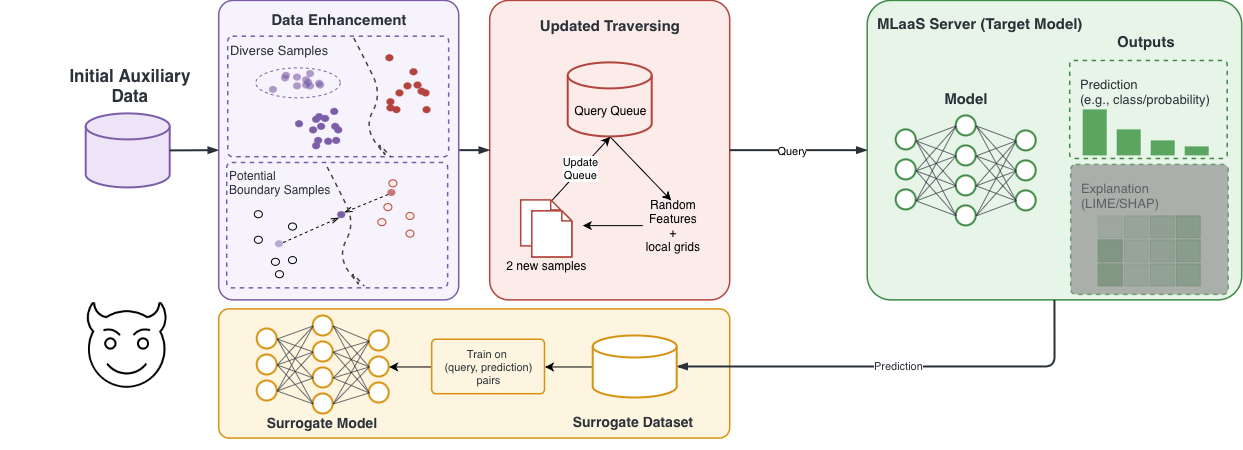
\includegraphics[width=\textwidth]{figures/extraction_pipeline-Page-2.drawio.png}
\caption{\sys. Phases~1 and~2 add diverse and boundary samples to a small seed set; Phase~3 steps
randomly chosen features from bin edges the adversary reads off a grid fitted on its \emph{own}
auxiliary data. The explanation endpoint (greyed) is never queried. The ablations of
\S\ref{subsec:e2}--\S\ref{subsec:e3} read it instead.}
\label{fig:pipeline}
\end{figure*}

Figure~\ref{fig:pipeline} sketches the pipeline. \sys\ builds on the Autolycus traversal, which
expands a small per-class seed set one feature at a time: it picks a \emph{base coordinate} for a
selected feature and emits two children, one at each of base ${}\pm{}\varepsilon_i$, where
$\varepsilon_i$ is a fixed per-feature step scaled to feature $i$'s spread. Which coordinate serves
as the base is precisely what the explainer supplies: \textsc{Lime} offers a bin edge and
\textsc{Shap} offers nothing, leaving the feature's current value
(\S\ref{subsec:traversal}). Like a bin edge, $\varepsilon_i$ is a distributional statistic, so the
adversary can set it from its own auxiliary sample.

The three phases can be driven with either explainer $\mathcal{E} \in \{\textsc{Shap},
\textsc{Lime}\}$, and the two instantiations differ \emph{only} where the discretization threshold
enters the computation (Phase~2 placement and Phase~3 stepping). The bin-edge stepping that
constitutes \textsc{Lime}'s threshold channel is Autolycus's \emph{own} mechanism, retained unchanged
rather than introduced by us. Holding everything else fixed turns the
\textsc{Shap}-versus-\textsc{Lime} comparison into a controlled experiment that isolates the threshold
channel (\textbf{H2}), while ablating the explanation's feature choice isolates the attribution
channel (\textbf{H1}).

A variant reading the target's \textsc{Lime} output instead of a self-computed grid lets query
\emph{placement} be compared against Autolycus at equal information access
(\S\ref{subsec:e4}, Appendix~\ref{app:decomp}). The channel ablations are separate again: they run on
the \emph{base} Autolycus traversal, so those conclusions do not depend on our additions.
Algorithm~\ref{alg:attack} summarises the three phases.

\begin{algorithm}[t]
\caption{Boundary-directed extraction with explainer
$\mathcal{E}\in\{\textsc{Shap},\textsc{Lime}\}$. Parameter values are given in
\S\ref{subsec:diverse}--\ref{subsec:traversal}.}
\label{alg:attack}
\begin{algorithmic}[1]
\Require target $f$, explainer $\mathcal{E}$, seeds $\mathcal{D}_0$, budget $Q$
\Ensure surrogate $\hat{f}$
\State $\mathcal{S}, \mathcal{T} \gets \mathcal{D}_0$
       \Comment{traversal queue, labelled set}
\Statex \textit{// Phase 1: diverse query generation}
\State $\mathcal{S} \gets \mathcal{S} \cup
       \{x \in \textsc{DiverseGen}(\mathcal{S}) \,:\, \max \hat{p}(x) > \tau\}$
       \Comment{$\mathcal{E}$ used only by the \textsc{Lime}-threshold variant}
\Statex \textit{// Phase 2: boundary search}
\For{$n_{\text{mid}}$ cross-class pairs $(a,b)$ drawn from $\mathcal{S}$}
  \State $c \gets a$ with its top-$k_b$ features moved toward $b$
         \Comment{\textsc{Lime}: to the bin edge; \textsc{Shap}: midpoint}
  \State $(c, M) \gets \textsc{Bisect}(c, b)$ \Comment{$8$ steps, midpoints $M$}
  \State $\mathcal{S} \gets \mathcal{S} \cup \{c\}$;\quad $\mathcal{T} \gets \mathcal{T} \cup M$
\EndFor
\Statex \textit{// Phase 3: explanation-guided traversal}
\While{$\mathcal{S} \neq \emptyset$ \textbf{and} budget and per-class quotas remain}
  \State $x \gets \textsc{Pop}(\mathcal{S})$;\quad $\mathcal{T} \gets \mathcal{T} \cup \{(x, f(x))\}$
  \ForAll{$i$ among the top-$k$ features of $x$ by $\mathcal{E}$}
     \State add $x$ with coordinate $i$ stepped by $\pm\varepsilon_i$, if valid and new
            \Comment{\textsc{Lime}: from the bin edge}
  \EndFor
\EndWhile
\State \Return $\hat{f} \gets \textsc{Train}(\mathcal{T})$
\end{algorithmic}
\end{algorithm}

\subsection{Phase 1: Diverse Query Generation}
\label{subsec:diverse}
Autolycus seeds its traversal from a handful of per-class points and expands them by
local perturbation, which tends to under-cover behavioural regions the seeds never
reach. Phase~1 counters this with one of two generators, both returning \emph{unqueried}
candidates that are then queried and kept only if confidently classified
($\max \hat{p}(x) > \tau$ with $\tau = 0.8$):
\begin{itemize}
  \item \textbf{Plausibility-filtered} (explanation-free): crossover and mutation of the current
  pool produce a large candidate set, of which those further from the seeds than the $90$th
  percentile of the seeds' own nearest-neighbour distances are rejected as off-manifold. The
  survivor furthest from everything kept so far is then added to the pool, and the step repeats. This
  is a greedy max--min (k-center) selection in input space, purely geometric and using no model
  output beyond the confidence filter above.
  \item \textbf{LIME-threshold} (explanation-informed): harvest the target's LIME
  bin-edge thresholds from the seed explanations, synthesise
  seed-anchored candidates that \emph{cross} those thresholds into different decision
  cells, plausibility-filter them, and greedily select the candidates covering the most
  distinct $(\text{feature}, \text{threshold}, \text{side})$ configurations. If the
  target surfaces no thresholds (e.g.\ a linear model), it falls back to the geometric
  generator.
\end{itemize}
In its plausibility-filtered form Phase~1 uses no explanation information at all, and this is the
form \sys\ runs. The \textsc{Lime}-threshold variant uses both channels: the ranking decides whose
thresholds are harvested (only the top-$k$ features of each seed explanation are read), and the
thresholds themselves drive the crossing.

\subsection{Phase 2: Boundary Search}
\label{subsec:boundary}
Phase~2 places training points \emph{on} the decision boundary, where labels are most
informative. We enumerate the cross-class pairs available among the current samples, shuffle them,
and draw $n_{\text{mid}}$ of them without replacement (refilling the pool if it empties). For each
drawn pair $(a,b)$ we build a child from $a$ by blending its top-$k_b$ features toward $b$, then run
an $8$-step bisection between the child and $b$ to converge onto the boundary between their classes.
Enumerating every pair would be quadratic in the seed count and would exhaust the budget on this
phase alone, so $n_{\text{mid}}$ is a parameter ($10$ by default, reduced at small $Q$ so Phase~3 is
not starved). The explainer governs \emph{how} the
child is placed, and this is precisely where the threshold channel enters:
\begin{itemize}
  \item \textbf{\textsc{Lime}} snaps each continuous top-$k_b$ feature to its local
  \emph{bin edge} on the side toward $b$, a direct, free estimate of where the boundary
  crosses that coordinate.
  \item \textbf{\textsc{Shap}}, having only magnitudes, places the blend at the
  \emph{midpoint} and must rely on the subsequent bisection to \emph{search} for the
  same boundary location.
\end{itemize}
The bisection midpoints are recycled into $\mathcal{T}$ as boundary-concentrated training data,
and are not $\varepsilon$-perturbed further.

\subsection{Phase 3: Explanation-Guided Traversal}
\label{subsec:traversal}
Phase~3 is the Autolycus-style expansion. We pop a sample $x$, query and label it,
explain it with $\mathcal{E}$, rank its features by $|\phi_i|$ (\textsc{Shap}) or $|w_i|$
(\textsc{Lime}) and keep the top $k$, then emit two children per selected feature $i$, stepped by
$\pm\varepsilon_i$. The attributions choose \emph{which} coordinates move; $\varepsilon_i$ sets how far. Valid, non-duplicate children re-enter the queue until the budget is
exhausted or all classes are sufficiently visited. We retain this expansion because it matters on its own (removing Phase~3 degrades fidelity, most sharply for tree targets), but the \emph{attribution-based selection} is \emph{not} what drives it:
consistent with \textbf{H1}, replacing the explanation's top-$k$ choice with a random one
leaves fidelity essentially unchanged on our primary (non-tree) targets
(\S\ref{subsec:e2}). What differentiates the two explainers here is, once more, the
threshold channel: \textsc{Lime} steps $\pm\varepsilon_i$ \emph{from the feature's bin edge}, so each step crosses the local threshold, whereas \textsc{Shap} steps from the
current value using only the attribution ranking. Phase~3 therefore contributes
coverage and expansion. Its sole explanation-supplied benefit is \textsc{Lime}'s
threshold stepping, not the attribution ranking.

% =======================================================================
\section{Experiments}
\label{sec:experiments}
\subsection{Setup}
\label{subsec:setup}
We evaluate on six public tabular datasets (Table~\ref{tab:datasets}) covering continuous,
categorical, and mixed feature schemas, against five target families: logistic regression (LR), naive
Bayes (NB), $k$-NN, decision tree (DT) and random forest (RF). All five appear in every experiment: the channel
ablations of \S\ref{subsec:e2} and \S\ref{subsec:e3}, the self-computability test of
\S\ref{subsec:e5}, in the adversary comparison of \S\ref{subsec:ladder} and in the budget sweep. We scope to tabular data throughout,
following the attack we analyse~\cite{oksuz2024autolycus}. Following the Autolycus convention, the
LIME attacker uses $n{=}1$
seed per class and explores $k{=}3$ top features, and the SHAP attacker uses $n{=}5$ and $k{=}3$.
Query budgets are per dataset (Table~\ref{tab:datasets}). We inherit the baseline's query
accounting unchanged: the explanation is bundled with the prediction and not charged separately, a
candidate already queried or queued is not resubmitted, and fidelity is reported against the query
\emph{budget} rather than queries consumed. Phases~1 and~2 both consume budget: every diverse
candidate is queried, including those the confidence filter then discards, and every bisection
midpoint is queried and retained as training data. A budget-scaling rule caps that combined overhead
so it cannot starve Phase~3 at small $Q$. Every arm we compare spends the same counted budget, so
\sys\ claims no advantage from the accounting.

Compared arms always run on \emph{paired} seed sets (identical draws, identical RNG state), and
surrogate fidelity (Eq.~\ref{eq:sim}) is aggregated by the \emph{mean} over refits. Significance is a
paired Wilcoxon signed-rank test over the $10$ paired observations, with $^{*}p{<}.05$ and
$^{**}p{<}.01$. With $10$ pairs the smallest attainable two-sided $p$-value is $2/2^{10}\approx.002$,
reached only when every pair falls the same way, so $^{**}$ marks a near-unanimous effect across
target instantiations rather than an arbitrarily small $p$.

\paragraph{Protocol.} We deviate from the original attack's reporting in two ways, both toward more
conservative estimates. \emph{Surrogate aggregation:} the original trains $R$ surrogate refits per
arm and reports the single one most similar to the target, a quantity measured on the evaluation set,
so the selection is made using the reported metric. We instead report the mean over the $R$ refits,
which is unbiased. ($R$ denotes surrogate refits and is unrelated to the top-$k$ feature budget $k$, and we use $R{=}20$ for DT, $R{=}10$ for RF, and $R{=}1$ otherwise.)
\emph{Target instantiation:} the original varies only the attacker's seed sets against a single fitted
target, so its reported spread reflects seed noise rather than variation across targets. For the
ablations (\S\ref{subsec:e2},~\S\ref{subsec:e3}) we therefore draw $10$ independent train/test splits
and retrain the target on each, pairing all arms within a split, so each observation is an independent
target instantiation. 
We retain the original single-split protocol only for the sweeps of
Appendix~\ref{app:matched} and Appendix~\ref{app:sweeps}, so that those numbers stay comparable to
the published baseline. Every comparison in the main text uses the multi-split protocol. 

\begin{table}[t]
\centering
\caption{Datasets. \emph{cont.} counts continuous features and $Q$ is the query budget. Train, evaluation
and auxiliary partitions follow the $75\!:\!15\!:\!10$ split of the attack we analyse.}
\label{tab:datasets}
\begin{tabular}{lrrrrr}
\toprule
 & $n$ & feat. & cont. & cls. & $Q$ \\
\midrule
crop      & $1{,}700$  & 7  & 7  & 17 & $1000$ \\
adult     & $32{,}561$ & 11 & 3  & 2  & $1000$ \\
breast    & $569$      & 30 & 30 & 2  & $100$  \\
nursery   & $12{,}960$ & 8  & 0  & 3  & $1000$ \\
mushroom  & $8{,}123$  & 21 & 0  & 2  & $1000$ \\
pendigits & $10{,}992$ & 16 & 16 & 10 & $1000$ \\
\bottomrule
\end{tabular}
\end{table}

\subsection{Is the attribution channel the leak? (H1)}
\label{subsec:e2}
Base Autolycus has two binary knobs: whether the top-$k$ features come from the explanation's ranking
or at random, and whether steps start from the exposed bin edge or from the sample's current value.
This section varies the first, \S\ref{subsec:e3} the second. We replace the explanation's top-$k$
feature selection with a random-$k$ choice, holding the rest of the attack fixed, and measure the
change in surrogate fidelity. If the attribution ranking carries exploitable signal, random selection should
be worse. Across both explainers the attribution channel is \emph{weak and inconsistent} ($S{=}10$
paired sets):
\begin{itemize}
  \item \textbf{\textsc{Shap}: no net advantage.} On the base Autolycus attack, SHAP-guided selection
  is \emph{no better on average} than random no-explanation traversal (Table~\ref{tab:shap-attr}: mean $-0.2$pp over $30$ cells, with $4$ significantly positive and $7$ significantly negative). Where it
  helps it is confined to \emph{tree} targets on datasets with a few dominant features, for which the
  \emph{exact} TreeSHAP pinpoints true splits (\textsc{mushroom} DT $+9.8$, RF $+6.9$pp, both
  $p{<}.01$). But the same explanation that helps trees on
  \textsc{mushroom} \emph{hurts} logistic regression on that very dataset ($-11.2$pp), and it misleads
  across the board on \textsc{nursery} (LR $-10.2$, NB $-9.1$, KNN $-4.6$pp). The sign of the effect is
  a property of the target, not of the explanation, so an attacker choosing to consult SHAP has no way
  to know whether doing so will help or harm.
  \item \textbf{\textsc{Lime}: no systematic advantage either.} Replacing \textsc{Lime}'s ranking with a random choice, holding the threshold available to both arms, changes fidelity by a mean of
  $-0.6$pp and a median of $-1.0$pp over the same $30$ cells, with $4$ significantly positive and $5$
  significantly negative (Table~\ref{tab:lime-attr}). This is weaker than claiming the channel is empty: individual cells
  show real effects, but their sign is not predictable from the dataset or the target family, so an
  attacker gains nothing it can rely on. The instability is itself informative: individual cells move
  by several points under changes that affect only \emph{which} features the control happens to draw,
  which is what one expects when the quantity being measured is close to zero.
\end{itemize}
So neither explainer's attribution ranking confers a systematic extraction advantage. This is not
merely an absence of significance: the contrast with the \emph{threshold} channel is \emph{directional}.
Over the identical cells, threshold ablation is significantly positive twelve times and significantly
negative \emph{never} (mean $+6.7$pp), whereas attribution is significant in both directions, four
times positive against five negative, around a mean of $-0.6$pp (\S\ref{subsec:e3}). One channel has a sign, and the other does not.
What \textsc{Lime} supplies is not a useful feature ranking but a discretization \emph{threshold}.

\begin{table}[t]
\centering
\caption{Attribution ablation on the \emph{base} Autolycus \textsc{Shap} attack: fidelity gain
(points) from selecting top-$k$ features by \textsc{Shap} importance rather than at random ($n{=}5$,
$k{=}3$; $^{*}p{<}.05$, $^{**}p{<}.01$). Ten paired splits per cell. Negative $=$ random wins.}
\label{tab:shap-attr}
\setlength{\tabcolsep}{3pt}
\begin{tabular}{lrrrrrr}
\toprule
 & crop & pendigits & breast & adult & nursery & mushroom \\
\midrule
LR  & $-5.5^{*}$ & $-1.9^{*}$  & $+1.2$ & $-0.0$ & $-10.2^{**}$ & $-11.2^{**}$ \\
NB  & $-1.0$     & $+0.6$      & $+1.4$ & $+2.5$ & $-9.1^{**}$  & $+3.8$ \\
KNN & $+1.0$     & $+1.0$      & $-0.3$ & $+1.0$ & $-4.6^{**}$  & $+3.6^{*}$ \\
DT  & $+1.3$     & $+2.7$      & $+2.3$ & $+0.7$ & $-1.1^{*}$   & $+9.8^{**}$ \\
RF  & $+0.4$     & $-1.5$      & $+0.3$ & $+0.7$ & $+0.7^{*}$   & $+6.9^{**}$ \\
\bottomrule
\end{tabular}
\end{table}

\begin{table}[t]
\centering
\caption{Attribution ablation on the \emph{base} Autolycus \textsc{Lime} attack: fidelity gain (points) from selecting top-$k$
features by \textsc{Lime}'s ranking rather than at random, with the bin edge available to both arms
($n{=}1$, $k{=}3$; $^{*}p{<}.05$, $^{**}p{<}.01$). Ten paired splits per cell. $^{\dag}$ marks cells
with too few non-tied splits to test.}
\label{tab:lime-attr}
\setlength{\tabcolsep}{3pt}
\begin{tabular}{lrrrrrr}
\toprule
 & crop & pendigits & breast & adult & nursery & mushroom \\
\midrule
LR  & $-3.8^{*}$  & $+0.1$        & $+6.0$        & $-4.5$        & $-0.2$       & $-2.9$ \\
NB  & $+6.8^{**}$ & $-1.4$        & $+5.2$        & $-1.8^{\dag}$ & $-6.0$       & $-15.4^{*}$ \\
KNN & $+4.4$      & $-0.6$        & $+4.0^{\dag}$ & $-0.3$        & $+5.7^{**}$  & $+6.1^{*}$ \\
DT  & $-2.2$      & $-5.7^{*}$    & $-2.7$        & $-6.0$        & $+1.5$       & $+5.3$ \\
RF  & $-4.0$      & $-6.9^{**}$   & $-5.6$        & $-3.7^{**}$   & $+1.5^{*}$   & $+7.7$ \\
\bottomrule
\end{tabular}
\end{table}

\subsection{Is the threshold (bin edge) the leak? (H2)}
\label{subsec:e3}
We now vary the second knob, with the feature
choice fixed to \textsc{Lime}'s ranking: we perturb from the bin edge \textsc{Lime} exposes (default)
versus from the sample's current value (no-threshold), everything else identical. Because the base
attack already snaps to the bin edge and has \emph{no} boundary search to mask the effect, this is
the cleanest possible test of H2.

\begin{table}[t]
\centering
\caption{Threshold ablation on the \emph{base} Autolycus \textsc{Lime} attack: fidelity gain (points) from perturbing at the
exposed \emph{bin edge} rather than the current value, features held to \textsc{Lime}'s ranking
($n{=}1$, $k{=}3$; $^{*}p{<}.05$, $^{**}p{<}.01$, $^{\dag}$ too few non-tied splits to test). Same
protocol, cells and layout as Table~\ref{tab:lime-attr}. Positive $=$ the threshold helps.}
\label{tab:lime-threshold}
\setlength{\tabcolsep}{3pt}
\begin{tabular}{lrrrrrr}
\toprule
 & crop & pendigits & breast & adult & nursery & mushroom \\
\midrule
LR  & $+40.9^{**}$ & $+18.6^{**}$ & $-10.2$        & $-1.8$        & $-0.8$      & $-8.7$ \\
NB  & $+24.9^{**}$ & $+7.9^{**}$  & $+11.2^{*}$    & $+0.0^{\dag}$ & $+5.0^{**}$ & $-0.2$ \\
KNN & $+15.2^{**}$ & $+0.4$       & $-0.2^{\dag}$  & $-0.3$        & $+1.0^{**}$ & $+13.9^{**}$ \\
DT  & $+38.0^{**}$ & $+10.1^{*}$  & $+4.8^{\dag}$  & $+2.6$        & $+0.6$      & $+2.1$ \\
RF  & $+22.7^{**}$ & $+0.7$       & $+1.1$         & $+0.9$        & $+0.5$      & $-0.8$ \\
\bottomrule
\end{tabular}
\end{table}

\paragraph{The threshold channel is directionally consistent.} On the two datasets whose evaluation
sets can resolve it, the bin-edge signal produces large, significant gains: crop (agronomy, $+15$ to
$+41$pp) and pendigits (pen-trajectory, $+8$ to $+19$pp), across ten independent target
instantiations. The asymmetry is what matters: over these cells the threshold ablation is
significantly positive twelve times and significantly negative \emph{never}, whereas the attribution
ablation on the identical cells is significant in both directions
(Table~\ref{tab:lime-attr}). This is precisely the signal \emph{absent} from \textsc{Shap}: on
pendigits, \textsc{Lime}'s threshold yields $+8$ to $+19$pp while \textsc{Shap}'s attribution yields
$+2.7$pp (n.s.), because Shapley magnitudes carry no ``where'' information. H2 holds where H1 fails.

\paragraph{Scope: the mechanism predicts where the channel is weak.} The threshold channel is
load-bearing only when \textsc{Lime}'s per-feature bin edge is a meaningful proxy for the decision
boundary \emph{and} the base attack has room to improve. Both conditions bite. Where features are
\emph{categorical}, discretization yields few distinct cut points and the channel is correspondingly
weak and unstable: on \textsc{nursery} the effect is at most a few points against $+15$ to $+41$pp on
crop, and it does not reproduce reliably (the NB cell measures $+5.0$ in one run and $+1.0$ in another differing only in random seed). We report this rather than a clean null because
\textsc{nursery}'s features are label-encoded ordinals, so quartiles do fall on real level boundaries, but the channel there is too small to support a claim in either direction. Where the target is \emph{near-ceiling} (breast) there is
no headroom for any channel to exploit. We scope all experiments to tabular data, following the attack we extend. We therefore make no claim about high-dimensional or non-axis-aligned regimes.

\subsection{Is the threshold privileged to the target?}
\label{subsec:e5}
\S\ref{subsec:e3} establishes that the discretization threshold is the channel that matters. It does
not establish that the threshold is \emph{information the service discloses}. \textsc{Lime}'s default
\texttt{QuartileDiscretizer} places its bin edges at the $25/50/75$ percentiles of the explainer's background data, a statistic of the data distribution that is independent of the model and of the
labels. If an adversary can estimate those percentiles from data it already holds, the discretization
accelerates extraction without disclosing anything.

We test this directly on \textsc{Lime} itself. Holding the traversal, the seeds, and the RNG fixed, we
vary only the data the discretizer is fit on, across three paired arms: \texttt{nothresh} (no bin
edge), \texttt{tgt} (discretizer fit on the target's $X_{\text{train}}$, what the service exposes),
and \texttt{aux} (discretizer fit on the adversary's own auxiliary data). We report
$\text{thr}_{\text{tgt}}$ and $\text{thr}_{\text{aux}}$, each measured against \texttt{nothresh}, and
the privileged advantage $\text{leak}=\texttt{tgt}-\texttt{aux}$.

\begin{table}[t]
\centering\footnotesize
\setlength{\tabcolsep}{3pt}
\caption{How much auxiliary data the adversary needs to rebuild the grid. Every cell where the
threshold channel significantly helps ($p{<}.05$), ordered by effect size. Entries are fidelity gains
over a no-threshold baseline, using the target's own discretizer ($\text{tgt}$) or one the adversary
fits on $n$ samples \emph{per class} or on its full auxiliary partition.
$\text{leak}=\text{tgt}-\text{aux}_{\text{full}}$, negative favours the adversary, $^{*}p{<}.05$. Ten
paired splits, and $\text{tgt}$ reproduces Table~\ref{tab:lime-threshold}. The per-class sweep covers
the datasets with continuous features (\textemdash\ for the fully categorical ones, whose bin edges
are artefacts of the integer encoding, \S\ref{sec:discussion}).}
\label{tab:auxdisc}
\begin{tabular}{llr rrrr rr}
\toprule
& & & \multicolumn{4}{c}{$\text{aux}$, fitted on $n$ samples per class} & & \\
\cmidrule(lr){4-7}
dataset & model & tgt & $n{=}1$ & $n{=}2$ & $n{=}3$ & $n{=}5$ & aux$_{\text{full}}$ & leak \\
\midrule
crop      & LR  & $+40.9$ & $+40.7$ & $+43.9$ & $+40.9$ & $+42.8$ & $+41.9$ & $-0.9$ \\
crop      & DT  & $+38.0$ & $+38.2$ & $+38.2$ & $+38.6$ & $+37.3$ & $+36.8$ & $+1.1$ \\
crop      & NB  & $+24.9$ & $+23.4$ & $+23.4$ & $+24.5$ & $+24.1$ & $+24.1$ & $+0.9$ \\
crop      & RF  & $+22.7$ & $+20.5$ & $+20.7$ & $+23.4$ & $+22.1$ & $+22.4$ & $+0.3$ \\
pendigits & LR  & $+18.6$ & $+12.9$ & $+15.4$ & $+16.5$ & $+16.6$ & $+20.1$ & $-1.5$ \\
crop      & KNN & $+15.2$ & $+10.9$ & $+16.4$ & $+17.1$ & $+15.9$ & $+17.7$ & $-2.5^{*}$ \\
breast    & NB  & $+11.2$ & $+6.0$  & $+10.9$ & $+9.7$  & $+11.9$ & $+11.9$ & $-0.7$ \\
pendigits & DT  & $+10.1$ & $+9.3$  & $+9.3$  & $+10.9$ & $+10.6$ & $+13.5$ & $-3.4$ \\
pendigits & NB  & $+7.9$  & $+5.2$  & $+7.8$  & $+7.8$  & $+6.8$  & $+7.8$  & $+0.2$ \\
\addlinespace
\multicolumn{9}{l}{\emph{fully categorical: no continuous axis, so no per-class sweep}} \\
mushroom  & KNN & $+13.9$ & \multicolumn{4}{c}{\textemdash} & $+15.8$ & $-1.9$ \\
nursery   & NB  & $+5.0$  & \multicolumn{4}{c}{\textemdash} & $+4.7$  & $+0.3$ \\
nursery   & KNN & $+1.0$  & \multicolumn{4}{c}{\textemdash} & $+1.3$  & $-0.3$ \\
\bottomrule
\end{tabular}
\end{table}

\paragraph{The discretization helps, but it is not a disclosure.} Across all twelve cells in which the
threshold channel is significantly positive, spanning five datasets and every target family, the adversary's own discretizer reproduces the gain (Table~\ref{tab:auxdisc}): on crop,
$\text{thr}_{\text{aux}}$ reaches $+41.9$pp against $\text{thr}_{\text{tgt}}$'s $+40.9$pp, with
differences averaging $-0.7$pp and spanning $-3.4$ to $+1.1$pp against threshold effects of up to
$+40.9$pp. Exactly one leak term reaches significance, and it runs the wrong way for the service:
on crop/KNN the adversary's self-computed grid is \emph{better} than the target's own by $2.5$pp
($p{<}.05$). Elsewhere the sign is inconsistent, the self-computed grid being marginally better in
seven of the twelve cells, which is what one expects of two estimates of the same quantity rather
than of a degraded substitute.
The result covers continuous (crop, pendigits), near-ceiling (breast), and categorical (nursery) targets alike. The threshold channel is therefore a
\emph{self-computable} property of the data distribution rather than privileged information about the
model. This reframes the finding of \S\ref{subsec:e3}: what \textsc{Lime}'s discretization supplies is
a data-adaptive grid of candidate cut points that makes boundary-straddling queries cheap, valuable to an attacker, but not something the service is uniquely able to reveal.

\paragraph{How much auxiliary data this requires.} Self-computation is bounded by the quality of the
adversary's distributional estimate, and the threat model we inherit permits a range of auxiliary set
sizes~\cite{oksuz2024autolycus}. The result above fits the discretizer on the full auxiliary
partition, the ``comprehensive'' end of that range. To find the other end we sweep the number of
samples \emph{per class} the discretizer is fitted on, on the datasets with continuous features,
holding the attack, the seed set, the budget and the RNG fixed, so only the estimate of the grid
varies (Table~\ref{tab:auxdisc}).

The requirement is very small, and crop and pendigits bound it from either side. On crop the adversary
is at parity with \emph{one} sample per class, seventeen points against a $1{,}275$-row training set:
$+40.7$ against the target's $+40.9$ on LR, $+38.2$ against $+38.0$ on DT. Only KNN lags at $n{=}1$,
and it catches up by $n{=}2$. Pendigits converges more slowly, as its shape predicts: sixteen
wide-range continuous features to place quartiles on and ten classes rather than seventeen. Its tree
and generative targets are nonetheless at parity almost at once ($+9.3$ against the target's $+10.1$
on DT at one sample per class, $+7.8$ against $+7.9$ on NB at two), while LR climbs
$+12.9 \to +15.4 \to +16.5 \to +16.6$ and is still some two points short of the target's $+18.6$ at
five per class, closing only with the full partition.
The practical consequence is that the full auxiliary partition, which the threat model grants and
which the rightmost column uses, is not what the attack runs on. A quartile is a cheap statistic, and
a handful of points per class estimates it well enough to recover most of the gain: on crop the
columns to the left of $\text{aux}_{\text{full}}$ are, to within noise, the same numbers, and on
pendigits they reach $83$ to $100$ per cent of it.
An adversary holding a small fraction of that pool is therefore no worse off, so the result does not
depend on the generous end of the range we inherit. Re-estimating the bins online from the accumulated
query set is the one variant that does worse, because the attack concentrates queries near decision
boundaries and its own history is therefore a biased estimator of the marginal distribution the bins
summarise. What the adversary needs is a small \emph{representative} sample, and ``small'' means
single digits per class.



\paragraph{Why obfuscating the channel is unlikely to defend it.} Because the channel localises to \textsc{Lime}'s
\texttt{discretize\_continuous} step, disabling or coarsening it is the natural candidate mitigation.
Two caveats prevent us from claiming it as a validated defense. The first is the result above: the
grid is reconstructible, so withholding it removes a convenience rather than a capability. Second,
preliminary attempts to perturb the bins rather than remove them (more bins, rounded edges) did not
reduce extraction. Measuring what a defender actually gains by withholding or distorting the
discretization, against an adversary that adapts by self-supplying it, is left to future work.

% =======================================================================
\begin{table*}[t]
\centering
\caption{The adversary ladder. Fidelity (\%) for each adversary, then the three contrasts that carry
the argument. \textsc{sg}$-$\textsc{aut} is the disclosure comparison: it swaps the target's
explanation for the adversary's own grid at fixed phases. \textsc{defended} is the service that returns attribution weights but withholds the bin
edges. All arms share the counted budget $Q$, the auxiliary pool, the per-split seeds and the
evaluation set; ten independent target instantiations per cell, paired Wilcoxon, $^{*}p{<}.05$,
$^{**}p{<}.01$. \textsc{self-grid} and \sys\ issue zero explanation calls.}
\label{tab:ladder}
\begin{tabular}{llrrrrrrrr}
\toprule
& & \multicolumn{5}{c}{fidelity} & \multicolumn{3}{c}{contrast} \\
\cmidrule(lr){3-7}\cmidrule(lr){8-10}
dataset & model & \textsc{blind} & \textsc{defended} & \textsc{autolycus} & \textsc{self-grid}
& \sys & \textsc{sg}$-$\textsc{aut} & \sys$-$\textsc{aut} & \sys$-$\textsc{def} \\
\midrule
crop       & LR   & $38.9$ & $39.5$ & $80.4$ & $82.3$ & $91.6$ & $+1.8$ & $+11.1^{**}$ & $+52.1^{**}$ \\
crop       & NB   & $57.5$ & $56.0$ & $80.9$ & $72.7$ & $75.4$ & $-8.2^{**}$ & $-5.5^{*}$ & $+19.5^{**}$ \\
crop       & KNN  & $53.6$ & $51.4$ & $66.6$ & $61.4$ & $63.1$ & $-5.3^{*}$ & $-3.5$ & $+11.6^{**}$ \\
crop       & DT   & $40.0$ & $39.7$ & $77.6$ & $77.9$ & $89.9$ & $+0.3$ & $+12.3^{**}$ & $+50.3^{**}$ \\
crop       & RF   & $64.3$ & $59.5$ & $82.2$ & $86.1$ & $91.3$ & $+3.9^{*}$ & $+9.2^{**}$ & $+31.9^{**}$ \\
\addlinespace
pendigits  & LR   & $57.2$ & $48.9$ & $67.5$ & $70.3$ & $86.1$ & $+2.7$ & $+18.5^{**}$ & $+37.1^{**}$ \\
pendigits  & NB   & $66.7$ & $65.2$ & $73.1$ & $72.4$ & $84.1$ & $-0.8$ & $+11.0^{**}$ & $+18.9^{**}$ \\
pendigits  & KNN  & $62.5$ & $62.5$ & $62.8$ & $64.2$ & $68.9$ & $+1.4^{*}$ & $+6.1^{**}$ & $+6.4^{**}$ \\
pendigits  & DT   & $30.7$ & $32.6$ & $42.7$ & $48.2$ & $49.6$ & $+5.5$ & $+6.9^{*}$ & $+16.9^{**}$ \\
pendigits  & RF   & $47.6$ & $50.5$ & $49.8$ & $56.7$ & $73.4$ & $+6.9^{**}$ & $+23.6^{**}$ & $+22.9^{**}$ \\
\addlinespace
breast     & LR   & $68.9$ & $72.8$ & $62.6$ & $60.7$ & $78.0$ & $-1.9$ & $+15.4$ & $+5.2$ \\
breast     & NB   & $74.1$ & $75.6$ & $86.8$ & $80.7$ & $88.9$ & $-6.1$ & $+2.1$ & $+13.3^{*}$ \\
breast     & KNN  & $69.1$ & $71.7$ & $71.4$ & $66.2$ & $73.8$ & $-5.2$ & $+2.4$ & $+2.1$ \\
breast     & DT   & $63.8$ & $64.0$ & $68.8$ & $72.2$ & $73.4$ & $+3.4$ & $+4.6$ & $+9.4$ \\
breast     & RF   & $85.8$ & $75.5$ & $76.6$ & $85.3$ & $82.5$ & $+8.7^{**}$ & $+5.9$ & $+7.0$ \\
\addlinespace
adult      & LR   & $81.6$ & $81.3$ & $79.5$ & $85.1$ & $86.4$ & $+5.6^{**}$ & $+6.9$ & $+5.1$ \\
adult      & NB   & $87.8$ & $87.6$ & $87.7$ & $89.6$ & $89.9$ & $+2.0^{**}$ & $+2.2$ & $+2.2$ \\
adult      & KNN  & $82.8$ & $84.0$ & $83.8$ & $84.2$ & $86.7$ & $+0.4$ & $+3.0^{*}$ & $+2.7^{**}$ \\
adult      & DT   & $64.4$ & $68.4$ & $71.0$ & $75.1$ & $71.2$ & $+4.1$ & $+0.2$ & $+2.8$ \\
adult      & RF   & $81.0$ & $78.9$ & $79.8$ & $83.4$ & $87.5$ & $+3.6$ & $+7.8^{**}$ & $+8.6^{**}$ \\
\addlinespace
nursery    & LR   & $98.1$ & $98.7$ & $97.9$ & $98.1$ & $97.9$ & $+0.2$ & $+0.0$ & $-0.8^{**}$ \\
nursery    & NB   & $84.0$ & $79.1$ & $84.1$ & $90.4$ & $80.9$ & $+6.3^{**}$ & $-3.2$ & $+1.7$ \\
nursery    & KNN  & $69.0$ & $80.5$ & $81.5$ & $76.5$ & $71.0$ & $-5.0^{**}$ & $-10.5^{**}$ & $-9.5^{**}$ \\
nursery    & DT   & $87.1$ & $89.9$ & $90.5$ & $88.4$ & $88.7$ & $-2.0$ & $-1.8^{*}$ & $-1.2$ \\
nursery    & RF   & $86.2$ & $90.3$ & $90.8$ & $90.7$ & $88.7$ & $-0.1$ & $-2.1^{*}$ & $-1.6^{*}$ \\
\addlinespace
mushroom   & LR   & $85.3$ & $92.3$ & $83.6$ & $82.2$ & $80.8$ & $-1.4$ & $-2.8$ & $-11.5^{**}$ \\
mushroom   & NB   & $71.3$ & $65.8$ & $65.6$ & $76.8$ & $79.7$ & $+11.1$ & $+14.0^{*}$ & $+13.8^{*}$ \\
mushroom   & KNN  & $65.5$ & $63.7$ & $77.6$ & $72.6$ & $70.4$ & $-5.1^{*}$ & $-7.2$ & $+6.7$ \\
mushroom   & DT   & $72.3$ & $81.7$ & $83.7$ & $78.6$ & $77.3$ & $-5.2$ & $-6.5^{*}$ & $-4.4$ \\
mushroom   & RF   & $66.8$ & $81.5$ & $80.7$ & $74.1$ & $75.7$ & $-6.6$ & $-5.0$ & $-5.7^{*}$ \\
\midrule
\multicolumn{2}{l}{\emph{mean}} & $68.8$ & $69.6$ & $76.3$ & $76.8$ & $80.1$ & $+0.5$ & $+3.8$ & $+10.4$ \\
\bottomrule
\end{tabular}
\end{table*}

\subsection{What does the adversary need, and does withholding it help?}
\label{subsec:ladder}
The two channel ablations each remove one channel from the base attack. Composing them, and adding back the query
synthesis of \S\ref{sec:method}, yields the question this paper exists to answer: what does an
extraction adversary actually need, and how much of it does the service supply? We answer it with a
\emph{ladder} of four adversaries that differ only in what they are given. All four run the same
framework, the same counted budget, the same auxiliary pool, the same per-split seeds, the same
surrogate family and the same evaluation set:

\begin{itemize}
  \item \textsc{blind}: base traversal, random features, no grid. The floor.
  \item \textsc{autolycus}: base traversal with the target's explanation, its feature ranking \emph{and} its bin edges. The published attack.
  \item \textsc{self-grid}: base traversal, random features, bin edges from a discretizer the
  adversary fits on its own auxiliary sample. No explanation call is made.
  \item \sys (ours): \textsc{self-grid} plus Phase~1 diverse generation and
  Phase~2 boundary search. No explanation call is made.
\end{itemize}

Two of the contrasts this ladder supports answer different questions and should not be conflated.
\textsc{self-grid} versus \textsc{autolycus} holds the attack phases and the budget fixed and
replaces the explanation entirely, ranking and bin edges alike, with the adversary's own grid, so it
measures what explanation access is worth end to end. This is the privacy comparison;
\S\ref{subsec:e5} isolates the grid alone under tighter control and should be read alongside it. \sys\
versus \textsc{autolycus} varies the attack as well, so it measures attack strength rather than
disclosure. We report both and keep them apart.

Three contrasts carry the argument:
$\sys-\textsc{autolycus}$ (does the attack need the explanation endpoint at all?),
$\sys-\textsc{self-grid}$ (what do Phases~1--2 add on top of the same grid?), and
$\textsc{self-grid}-\textsc{autolycus}$ (does a self-computed grid substitute for the service's, at
equal phases?).

The two explanation-free arms make \emph{zero} calls to \texttt{explain\_instance}: the bin edges they
consume are read directly from the adversary's own discretizer, which is fit on its auxiliary pool
when the explainer is constructed and never touches the target.


\paragraph{The grid matters, but its source does not.} Compare \textsc{blind} against the two
grid-holding base-traversal arms. The grid is the largest single effect in the paper: on crop it moves
fidelity from $38.9$ to $82.3$ (LR) and $40.0$ to $77.9$ (DT), and it is what separates a usable
adversary from a hopeless one. But its \emph{source} does not matter. Across all thirty cells
$\textsc{self-grid}-\textsc{autolycus}$ averages $+0.5$pp with significance in both directions
(7 positive, 4 negative), and neither feature type shows a meaningful residual
($+1.2$pp on the continuous datasets, $-0.8$pp on the categorical ones, against threshold effects of
up to $+41$pp). An adversary that computes
its own discretization from an auxiliary sample is, to within noise, exactly as well off as one handed the target's explanation, and here that arm reads \emph{nothing} from the explanation, neither the
ranking nor the edges, so the substitution is complete rather than partial.

\paragraph{Which phase does the work.} A component-level decomposition
(Appendix~\ref{app:decomp}) separates the two additions. They contribute about equally on average
($+1.6$pp for boundary search, $+1.8$pp for diverse generation), but which dominates is
target-dependent in the way the weaknesses they address predict: naive Bayes gains almost entirely
from diverse generation (W1, $+6.4$pp), logistic regression and random forest almost entirely from
boundary search (W2, $+2.5$ and $+4.7$pp).

\paragraph{What the query-synthesis phases add.} The contrast
$\sys-\textsc{self-grid}$ isolates Phases~1--2 given an identical grid. It is
$+3.3$pp over all cells, and the aggregate hides a sharp and
mechanically predictable split: on the four datasets with continuous features it is $+5.9$pp with
\emph{nine significant gains and no significant losses}, while on the two fully categorical datasets it
is $-1.7$pp. The same split governs the comparison against the published attack:
$\sys-\textsc{autolycus}$ is $+7.0$pp (10 significant gains, 1 loss) on continuous data
and $-2.5$pp on categorical data.

The mechanism explains the boundary rather than excusing it. Phases~2 and~3 place queries by snapping
a feature to a bin edge. A purely categorical dataset has no continuous axis to discretize, so there
are no edges to snap to and the two phases degenerate to a random-feature traversal that is strictly
worse than following the explanation. This is the same scope condition that made the threshold channel
flat on adult in \S\ref{subsec:e3}, arriving from the other direction, and it bounds the attack
honestly: \emph{\sys\ is an attack on tabular targets with continuous features}. Where
that condition holds it dominates the explanation-guided baseline while querying no explanation at all. Where it does not, the explanation retains genuine value, most visibly on nursery/KNN, where
\textsc{autolycus} reaches $81.5$ against $71.0$ for \sys.

Neither part suffices alone: \textsc{autolycus} already holds a grid and is still beaten on
continuous data, while \textsc{blind} runs the same traversal without one and is far worse than
either. The gain is an interaction between bisection and grid-snapped coordinates.

\begin{figure*}[t]
\centering
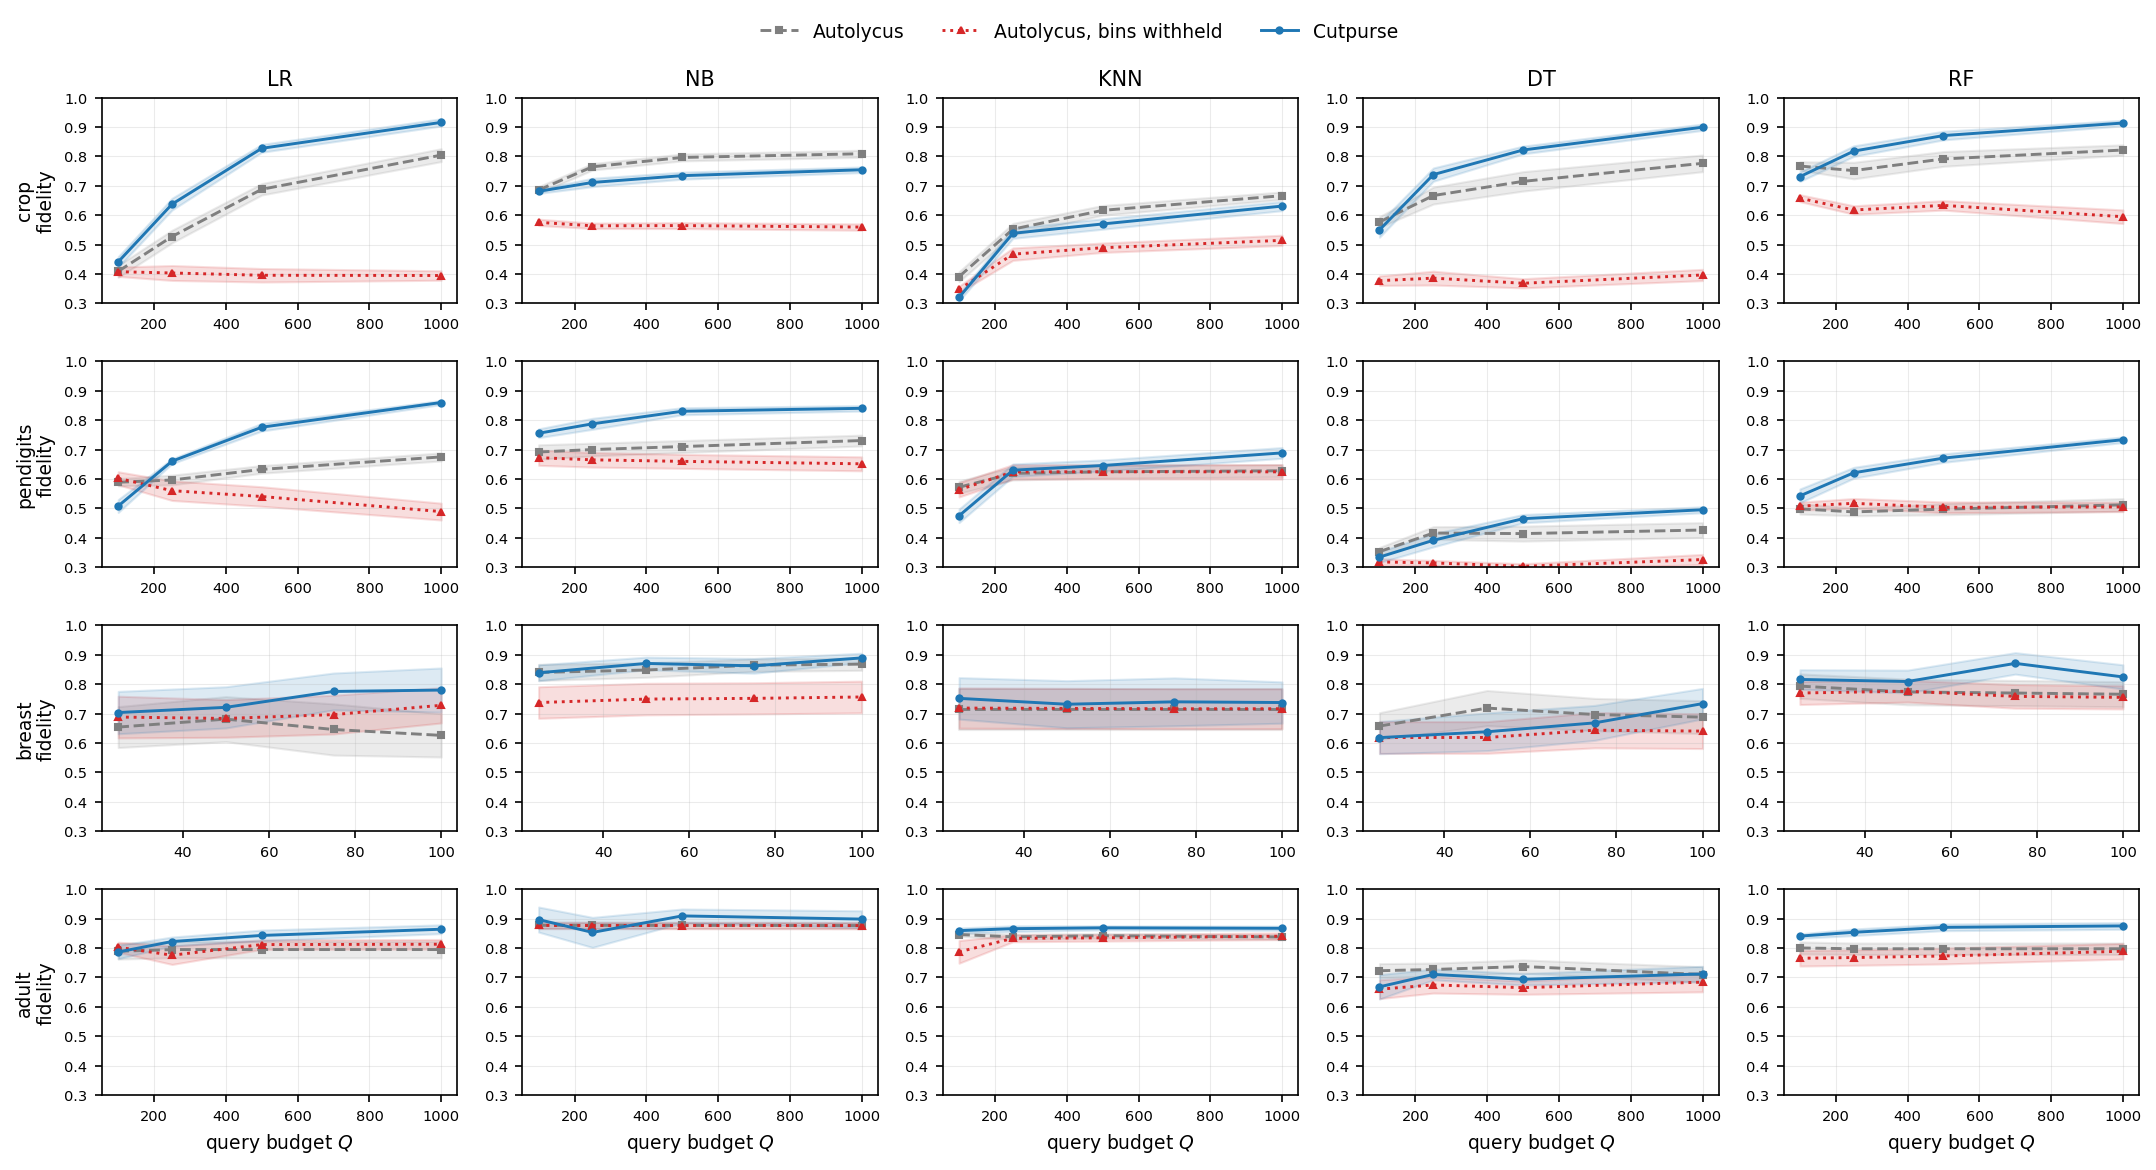
\includegraphics[width=0.72\textwidth]{figures/defense_sweep.png}
\caption{Fidelity vs.\ query budget for Autolycus (grey, dashed), Autolycus with bin edges
withheld (red, dotted) and \sys\ (blue, solid), per dataset (rows) and target (columns). The four
datasets with continuous features, the two purely categorical ones are
Figure~\ref{fig:defense-sweep-categ}. Band is the standard error over ten independent target
instantiations. Same splits, seed sets and attack RNG as Table~\ref{tab:ladder}, whose cells are the
rightmost point of each curve.}
\label{fig:defense-sweep}
\end{figure*}

\paragraph{Withholding the bin edges does not defend.}
\textsc{defended} is the service that returns attribution weights but suppresses the discretization,
the mitigation \S\ref{sec:analysis} derives from W3 and \S\ref{subsec:e3} shows is effective against
the attack it targets. On the ladder it is simply a rung below \textsc{autolycus}: removing the grid
moves the published attack down toward \textsc{blind}, collapsing crop/LR from $80.4$ to $39.5$ and
crop/DT from $77.6$ to $39.7$. It does not move \sys, which supplies its own grid and finishes
$+16.3$pp above the defended service on the four continuous-feature datasets, significant in thirteen
of twenty cells with no significant losses, reaching $+52.1$ and $+50.3$pp on the two crop cells the
defense hurt most.

\paragraph{The defense compounds rather than delays.}
A single budget cannot distinguish a defense from a speed bump: if withholding the bin edges only
slowed Autolycus down, the gap would close as the budget grew. Figure~\ref{fig:defense-sweep} shows
the opposite. The cost of the defense to Autolycus \emph{widens} monotonically with budget, from
$19.9$ to $38.0$pp on crop/DT and $11.0$ to $24.9$pp on crop/NB, and the pattern repeats on a second
dataset: on pendigits/LR the defense is worth nothing at $Q{=}100$ ($-1.4$pp) and $18.6$pp by
$Q{=}1000$. Bin-edge stepping is the
mechanism by which the traversal converts budget into boundary information. Withholding it does not
delay that conversion, it removes it. The distance from the defended service to \sys\ widens for the
same reason, reaching $+52.1$pp on crop/LR and $+50.3$pp on crop/DT at the largest budget.

Two features of the figure are worth stating rather than leaving to the reader. At the smallest
budget \sys\ is often \emph{behind} both baselines (crop/KNN $-7.1$, pendigits/LR $-9.4$pp at
$Q{=}100$): Phase~2 spends roughly $80$ queries on bisection, which at $Q{=}100$ is most of the
budget, and the curves cross by $Q{=}250$. And on pendigits/KNN the defense gap is flat at
approximately zero across every budget, one cell in which the threshold channel does no work at all.

Against an adversary of this kind the mitigation therefore buys none of what it was meant to buy: it
forfeits the transparency the explanation was published for and degrades the explanation for
legitimate users, while leaving achievable fidelity where it was. It may still be worth something
against an adversary with weaker auxiliary data, a regime we do not evaluate.

On the two purely categorical datasets we report no aggregate gain, and
Figure~\ref{fig:defense-sweep-categ} shows the reason rather than merely the outcome. There the
defense barely moves Autolycus either, the withheld and undefended curves lying on top of one another
at every budget, because the channel being withheld does not exist to withhold. On nursery \sys\
trails both baselines at every budget we test and converges toward them as the budget grows, ending
level with Autolycus on LR and still $10.5$ points behind on KNN. On mushroom the outcome is
target-dependent rather than uniformly negative: naive Bayes gains $+14.0$ against Autolycus while
KNN loses $7.2$. Neither the attack nor its mitigation is meaningful where there is no continuous
axis to discretize.

\section{Discussion and Limitations}
\label{sec:discussion}
\paragraph{Where the leak lives.} Our decomposition recasts explanation-guided extraction as a
question about \emph{discretization thresholds}. The exploitable signal is not the attribution magnitude
(\S\ref{subsec:e2}) nor, as prior framings imply, the boundary \emph{geometry}, but the discretization
threshold \textsc{Lime} publishes for free (\S\ref{subsec:e3}). \textsc{Shap}, which reports magnitude
without a threshold, carries no comparable signal \emph{on average}.

It does carry one in a specific and explicable case. Exact
TreeSHAP~\cite{lundberg2020treeshap} against a tree target is
significantly positive on \textsc{mushroom} (DT $+9.8$, RF $+6.9$pp, both $p{<}.01$), and the
mechanism is visible: for a tree the features with the largest attributions are
the ones tested at the split nodes, so a ranking computed exactly over that structure points at the
coordinates where the decision actually changes. That is the attribution channel approximating a
threshold rather than replacing it, and it does not generalise: the same explanation costs
$11.2$ points on logistic regression for the same dataset, because a linear target has no split nodes
for the ranking to recover. The practical consequence is still asymmetric: an MLaaS provider can serve
\textsc{Shap}-style magnitude attributions at substantially lower extraction risk than
\textsc{Lime}-style discretized explanations, with tree targets the case to watch.

A second consequence is about reach rather than risk. Because \sys\ never calls an explanation
endpoint, it is not restricted to services that publish explanations at all: the same attack runs
unchanged against an ordinary prediction API, which explanation-guided extraction cannot target. The
population of services exposed to this attack is therefore strictly larger than the population exposed
to the attack it derives from.

\paragraph{Scope and limitations.} The threshold channel is not universal, and we do not claim it is.
It is load-bearing only for continuous tabular targets with fidelity headroom (crop, pendigits). On
categorical features it is roughly an order of magnitude weaker, at most $+5$ to $+6$pp against
$+40.9$pp on crop, since discretizing a few ordinal levels yields few usable cut points, and on
near-ceiling targets it is absent because the attack is already saturated. We scope to tabular data throughout, following the attack we extend, and make no
claim about high-dimensional or non-axis-aligned domains.

\sys\ inherits the same boundary, and for the same reason: it places queries by snapping a feature to
a bin edge, so it operates only where that channel exists. The split reported in
\S\ref{subsec:ladder}, gains on the four continuous-feature datasets and none on nursery or mushroom,
is therefore what a missing channel predicts rather than an unexplained failure.

The categorical case deserves a sharper statement than ``the channel is weaker there,'' because the
bins on those datasets are not merely weak but \emph{spurious}. Following Autolycus, we construct
\textsc{Lime} without declaring which columns are categorical, so its discretizer treats every column
as continuous and places cuts at the quartiles of an integer label encoding. A ``bin edge'' on
mushroom is therefore a quantile of an arbitrary ordering of unordered categories, carrying no
information about any decision boundary. This predicts exactly what we observe: on those two datasets
the sign of every grid-related effect is inconsistent across targets (on mushroom the same grid is worth $+13.8$pp to naive Bayes and $-11.5$pp to logistic regression), which is the signature of an
artefact of the encoding rather than a channel. Note that this configuration is the
\emph{generous} one: had we declared the categorical columns, \textsc{Lime}'s discretizer would skip
them entirely and return equality rules of the form $\text{feature}{=}\text{value}$, leaving no bin
edge to snap to at all. Our setup therefore grants those datasets a threshold channel they would not
otherwise have, and it still does not help. We scope \sys\ to targets with genuine continuous
features and treat the categorical results as a negative control rather than a competitive
comparison.

The consequence for a defender is not symmetric with the consequence for an attacker: the
substitutability result of \S\ref{subsec:e5} holds on \emph{all} six datasets, so withholding
explanations does not protect a categorical-feature service either. It merely leaves \sys\ without an
edge to exploit.

\paragraph{Comparison with prediction-only extraction.} We do not benchmark \sys\ against a
published prediction-only attack such as Knockoff Nets or
\textsc{ActiveThief}~\cite{orekondy2019knockoff,pal2020activethief}, which draw their queries from a
large unlabelled transfer pool while the threat model we inherit grants $n{\le}5$ seeds per class, so
a matched-budget comparison would measure data assumptions rather than query strategy. The contrast
our question needs is already present under another name: \textsc{blind} runs the same traversal with
no grid and no explanation call, and \sys\ queries no explanation endpoint either. For Autolycus the
positioning against non-explanation extraction was established by its own authors, who benchmark it
against Tram\`er~et~al.'s path-finding and equation-solving attacks and against active-learning
extraction~\cite{tramer2016stealing,chandrasekaran2020active}.

Two measurement caveats bound what our per-cell numbers can support. First, \emph{evaluation-set size}
governs resolution: fidelity on \textsc{breast} is measured over $85$ held-out points, so one point is
worth $1.18$pp, against $255$ for crop ($0.39$pp) and $1648$ for pendigits ($0.06$pp). Effects of a few
points are therefore not resolvable on \textsc{breast}, and we rest no claim on it, a caution that
applies equally to prior work reporting per-cell fidelity on small splits. Second, the
crossing-rate objective in Phase~1 is a proxy for decision-cell coverage.

\section{Conclusion}
Explanation-guided extraction against interpretable tabular classifiers does not depend on the part of
the explanation that is specific to the model. Ablating each channel separately shows the attribution
ranking, in both \textsc{Lime} and \textsc{Shap}, confers no systematic advantage, being centred on
zero and inconsistent in sign. What carries the attack is the discretization threshold \textsc{Lime}
exposes as a bin edge, worth up to $41$ fidelity points and directionally consistent.

That threshold is a quantile of the background distribution rather than a property of the model, which
makes the obvious mitigation self-defeating. A service that withholds the bin edges costs the
published attack most of its advantage, but an adversary holding a representative auxiliary sample
estimates an equivalent grid and recovers it. We demonstrate this with \sys, which queries no
explanation endpoint at all: against the defended service it gains $+16.3$ fidelity points on targets
with continuous features, against the undefended service $+7.0$, and the margin over the defended
service \emph{widens} with budget rather than closing, because withholding the bin edges removes the
mechanism by which the traversal converts queries into boundary information. Because it needs no
explanation, the attack also applies to ordinary prediction APIs, which explanation-guided extraction
cannot target at all.

The practical reading for a provider is that suppressing explanations is the wrong lever against an
adversary that holds auxiliary data of its own. It forfeits the transparency the explanation was
published for and leaves that adversary no worse off, because the withheld quantity was never the
provider's to keep. Against an adversary without such data the lever may still do something, and
locating that crossover is the experiment we would run next. Where the attack does not apply is where the
channel does not exist: on purely categorical targets there are no meaningful cut points, and there
\sys\ shows no gain. Characterising what a defender can withhold that an adaptive adversary cannot
reconstruct remains open.

% ==== Back matter (outside the 12-page main body) ====
\appendix


\begin{ethics}
This work studies an \emph{attack} (model extraction guided by post-hoc explanations) in order to characterise a concrete privacy risk of explainable
machine-learning services. All experiments use publicly available benchmark
datasets and target models that we train ourselves. No proprietary system, personal data,
or live service was queried, and no human subjects were involved. The techniques extend
already-published extraction attacks and are evaluated in a controlled setting, so we
assess the incremental disclosure risk as low. Our findings are, on balance,
risk-\emph{reducing}: we show that the model-specific content of an explanation contributes
little to extraction, and that the component which does contribute is one an adversary can
reconstruct without the service's help. This bounds the incremental risk that publishing an
explanation creates, rather than expanding it. The work was not submitted to an external ethics board, as it involves no
human-subjects or live-system experimentation.
\end{ethics}

\begin{openscience}
We will release our attack implementation and evaluation harness, together with scripts
to reproduce every figure and table, upon acceptance. All datasets used are already public.
% BEFORE SUBMISSION: add an anonymised artifact link (e.g. anonymous.4open.science) here for review.
\end{openscience}

\begin{ai}
AI-based tools were used to assist with drafting and revising the text (improving flow and
correcting phrasing), to help search for related work, and for pre-submission review. The
authors have manually verified, and are responsible for, the accuracy, originality, and
integrity of all content, including every technical claim, experiment, and citation.
\end{ai}

\bibliographystyle{ACM-Reference-Format}
\bibliography{references}

% ==== Appendices: after the bibliography, per the PoPETs template ====
\section{Component decomposition: which phase drives the gain?}
\label{app:decomp}
\label{subsec:e1}
Our pipeline adds two components to the Autolycus traversal: diverse query generation (Phase~1) and
boundary search (Phase~2). We isolate their contributions with three nested arms on the same seed sets, namely Autolycus alone (\texttt{base}), $+$boundary (Phase~2, no diverse), and $+$diverse on top, so that boundary$\,=\,$($+$boundary)$\,-\,$\texttt{base} and
diverse$\,=\,$full$\,-\,$($+$boundary). Figure~\ref{fig:decomp} reports the result.

The two components contribute about equally on average ($+1.6$ and $+1.8$pp), but \emph{which} one
drives the gain is strongly target-dependent: naive Bayes benefits almost entirely from
\emph{diverse generation} ($+6.4$pp), since a generative model needs distribution coverage, whereas random forest and logistic regression benefit almost entirely from \emph{boundary search}
($+4.7$, $+2.5$pp), which places labelled points on the decision surface. In every case the gain is
query \emph{placement}, not the attribution ranking: consistent with H1, the components determine
\emph{where} queries land, and (\S\ref{subsec:e2}) replacing the explanation's feature ranking with a random one
does not systematically change fidelity. One caveat bounds this decomposition: the boundary term as
measured here bundles Phase-2 boundary search with the Phase-3 threshold stepping it inherits from
Autolycus, so it should be read as the combined contribution of both rather than of bisection alone.
\S\ref{subsec:e3} isolates the threshold component directly. Like the sweeps of Appendix~\ref{app:matched}, this decomposition uses the
explanation-reading configuration, so it measures what the two components add \emph{given} the
target's explanation, while \S\ref{subsec:ladder} measures what they add without it.

\begin{figure}[t]
\centering
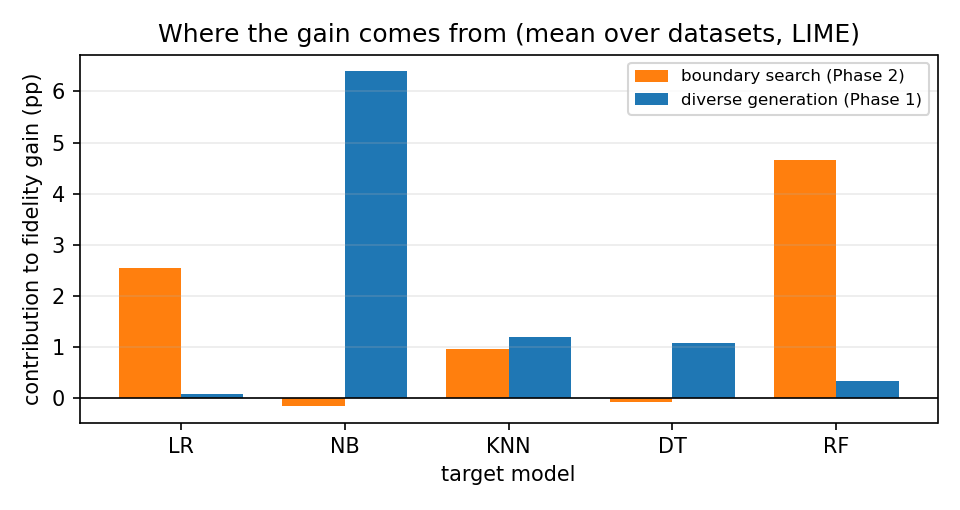
\includegraphics[width=0.9\linewidth]{figures/decomposition.png}
\caption{Contribution of each component to the LIME fidelity gain over
Autolycus (percentage points, mean over datasets, top budget). Boundary search dominates for
RF/LR; diverse generation dominates for NB.}
\label{fig:decomp}
\end{figure}

The split is also strongly \emph{dataset}-dependent (Figure~\ref{fig:decomp-perdataset}): diverse
generation carries almost the entire gain on \textsc{adult}/NB ($+34$pp, a generative target starved
of coverage), while boundary search dominates on the tree targets of \textsc{crop} and the linear
targets of \textsc{breast}. Neither component is tied to a particular dataset, both being query \emph{placement} mechanisms, which is why the aggregate in Figure~\ref{fig:decomp} splits evenly.

\begin{figure*}[t]
\centering
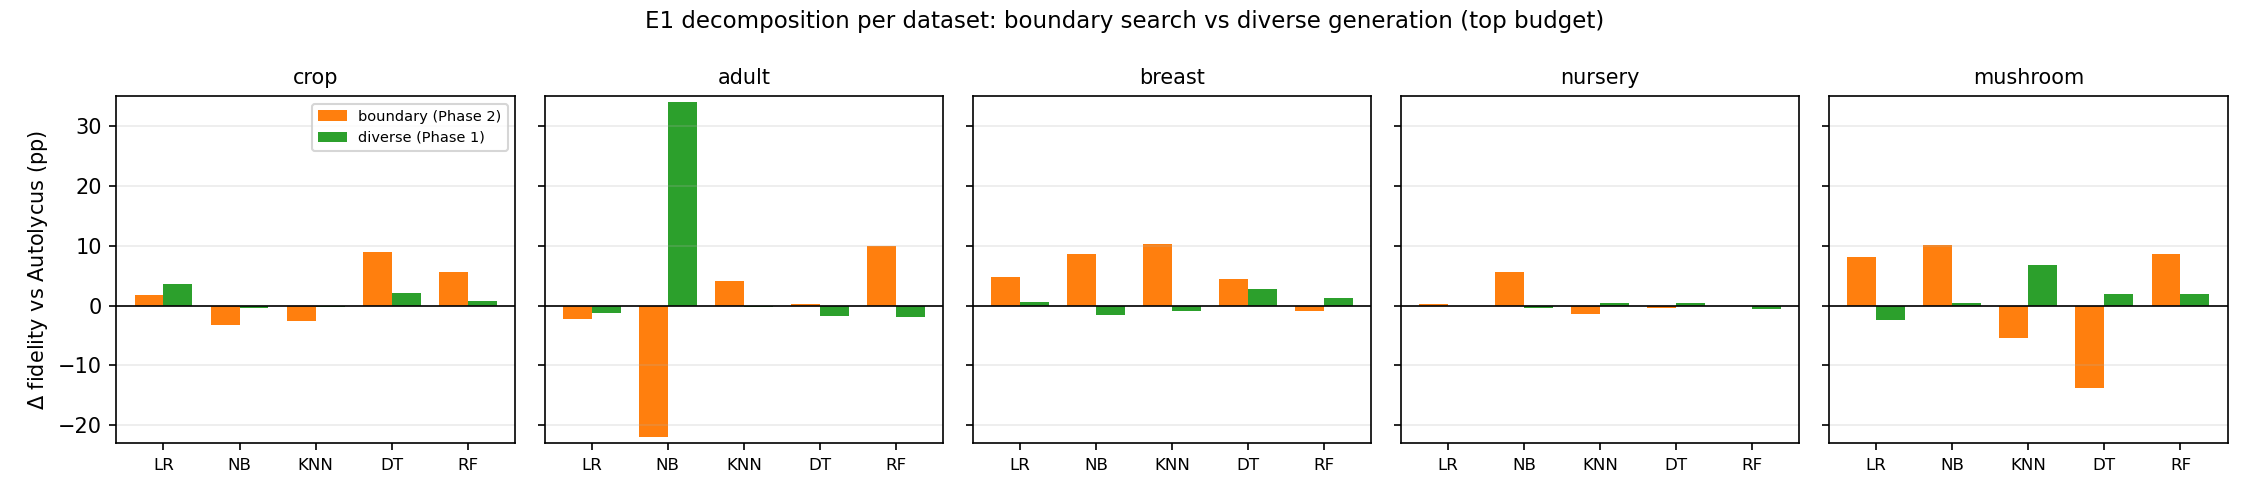
\includegraphics[width=\textwidth]{figures/decomposition_per_dataset.png}
\caption{Per dataset: contribution of boundary search (Phase~2, orange) and
diverse generation (Phase~1, green) to the LIME fidelity gain over Autolycus (percentage points, top
budget, mean over $S{=}10$ seed sets), one panel per dataset, grouped by target model. Shared
$y$-axis; the \textsc{adult}/NB diverse bar ($+34$pp) sets the scale.}
\label{fig:decomp-perdataset}
\end{figure*}

\section{Attack performance under matched information access}
\label{app:matched}
\label{subsec:e4}
This experiment runs our three phases with the target's explanation rather than a self-computed
grid, so both sides read the same \textsc{Lime} output and the comparison isolates query
\emph{placement}. \S\ref{subsec:ladder} evaluates the
\sys\ attack, which is the one the paper proposes.

Figure~\ref{fig:lime-headline} plots surrogate fidelity against query budget for the
explanation-reading configuration and the Autolycus \textsc{Lime} baseline. At a single
fixed diverse budget it improves fidelity on 18 of 25 target/dataset combinations (10 significant at
$p{<}.05$, against 2 significant regressions), with the most consistent gains on the non-tree targets
that have headroom (LR/NB on crop, nursery, and mushroom).

Establishing that the added phases are worth their budget is what licenses the null results that
follow: a channel that fails to help \emph{this} adversary is not failing for want of a capable
attack.

Part of this margin is an accounting effect worth stating plainly. Autolycus's traversal terminates
when its queue empties, which on several targets happens well before the budget is exhausted. Its curve then flattens because it \emph{cannot} spend the remaining budget, not because additional
queries would not help. Our Phase-1 and Phase-2 components keep generating admissible queries, so they
continue to convert budget into fidelity. Read at equal \emph{budget} the comparison therefore
flatters this configuration, and read at equal \emph{consumed queries} it would flatter Autolycus. We plot budget because that is the baseline's convention and the quantity a defender actually meters. The
$k{=}3$ control in Appendix~\ref{app:robustness}, where the baseline does spend its full budget,
isolates how much of the margin is saturation rather than better placement.

\begin{figure*}[t]
\centering
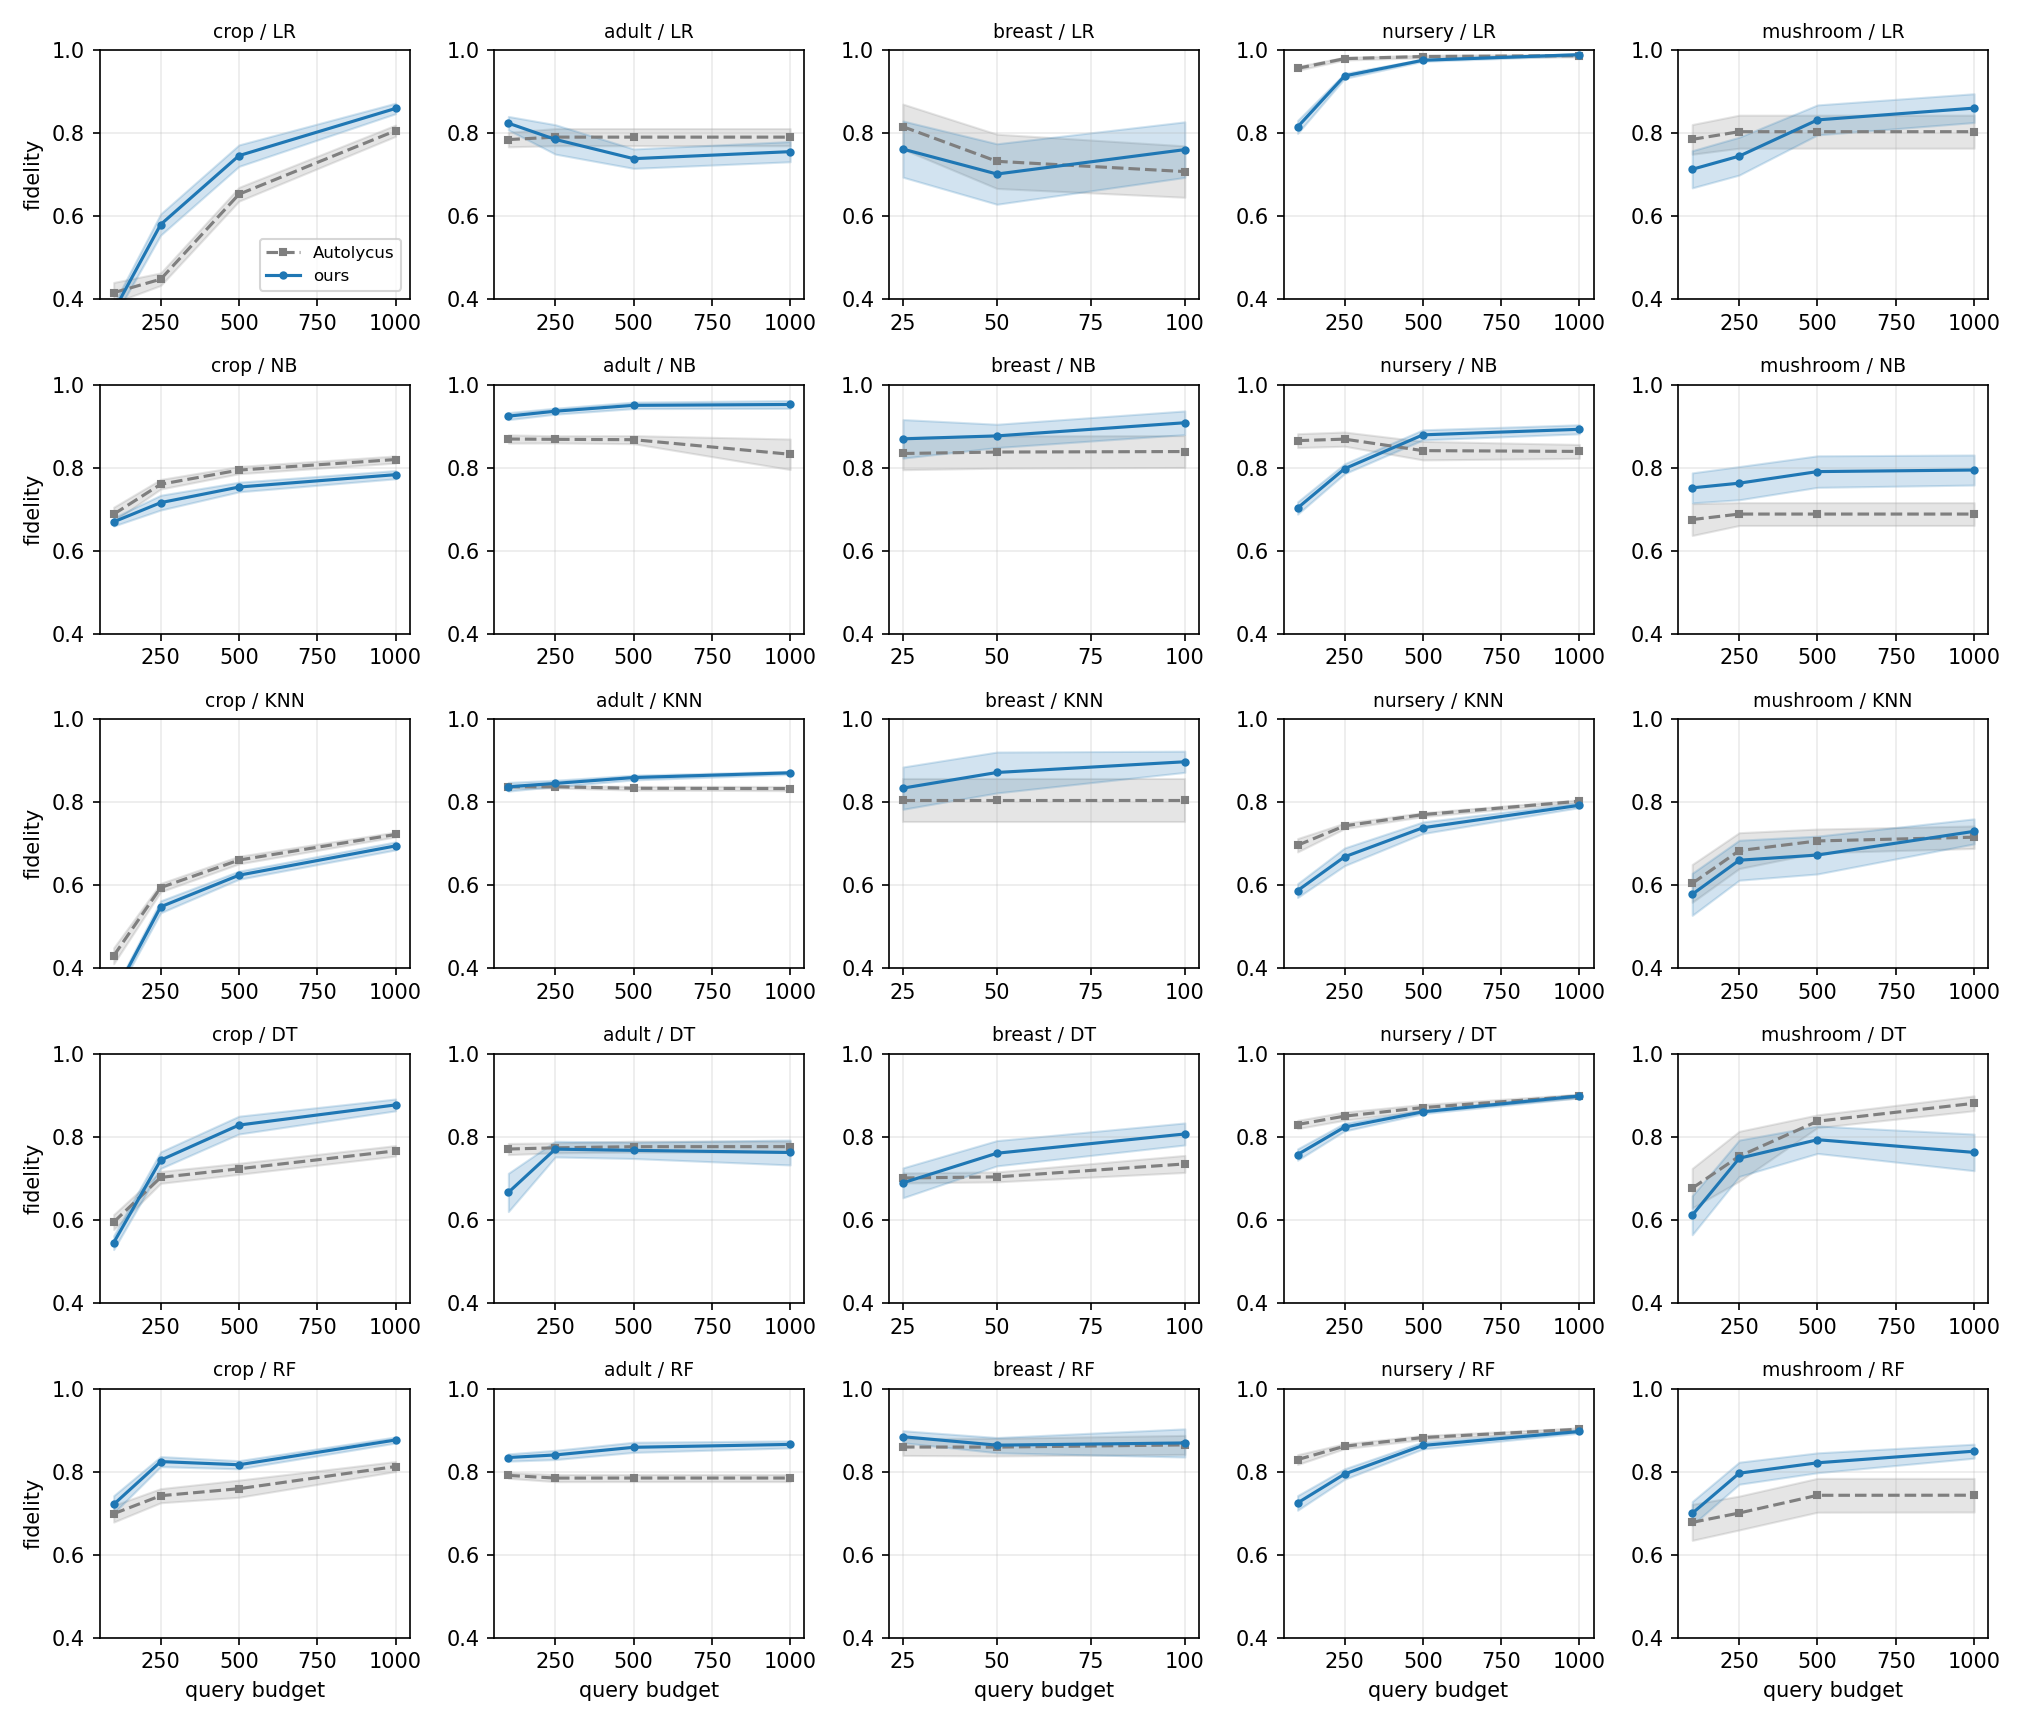
\includegraphics[width=\textwidth]{figures/lime_grid.png}
\caption{Fidelity vs.\ query budget, our phases reading the target's explanation (solid, blue) vs.\ Autolycus-\textsc{Lime}
(dashed, grey), per target (rows) and dataset (columns). Band is the standard error over $S{=}10$ seed
sets; $n{=}1$, $k{=}3$, diverse budget fixed at cap${=}15$. Shared $y$-axis ($0.4$--$1.0$).}
\label{fig:lime-headline}
\end{figure*}

\paragraph{The same attack helps under SHAP.}
Repeating this with \textsc{Shap} as the explainer ($n{=}5$, $k{=}3$) gives the same picture: the
same configuration improves over Autolycus-\textsc{Shap} on the same non-tree targets (LR/NB/KNN,
largest where the baseline has headroom, e.g.\ nursery and mushroom), while tree targets sit near
their fidelity ceiling and show no gain (Figure~\ref{fig:shap-headline}, Appendix~\ref{app:sweeps}).
That the same boundary-and-diversity machinery helps under \emph{both} explainers, independent of the particular attribution scores it consumes, is the first indication that the attribution channel is
not what drives the gain (H1). The \textsc{Lime}-specific advantage of a free \emph{threshold} is
isolated separately in \S\ref{subsec:e3}.

\paragraph{Diverse-budget sensitivity.}
The diverse generation (Phase~1) is regime-dependent: its optimal budget is roughly bimodal,
helping monotonically on high-headroom targets (best at the maximum budget, e.g.\ NB/adult:
$0.61{\to}0.96$ from no-diverse to full) and hurting on near-ceiling or small continuous targets
(best with no diverse). Because the budget is not the contribution, the headline figure fixes it
to a single value (cap${=}15$, the best global choice: $+3.4$pp mean, 18/25 wins) rather than
tuning per target. Fixing it this way costs accuracy on the targets that prefer a different budget,
and we prefer that cost to a per-target tuning that would not be available to a real attacker.

\section{Query-budget sweeps}
\label{app:sweeps}
\label{app:robustness}
This appendix collects the fidelity-versus-budget sweeps that compare our pipeline against Autolycus.
All of them run our phases with the target's explanation rather than a self-computed grid, so both
sides read the same output. The \sys\ attack is evaluated in \S\ref{subsec:ladder}.

Figure~\ref{fig:shap-headline} is the \textsc{Shap} companion to Figure~\ref{fig:lime-headline},
discussed in \S\ref{subsec:e4}. The remaining two vary \textsc{Lime}'s seed count and feature budget:
the main experiments use $k{=}3$, $n{=}1$ (the Autolycus setting), and we report here two alternative
settings under the identical protocol and fixed diverse budget of the main text.

\begin{figure*}[tbp]
\centering
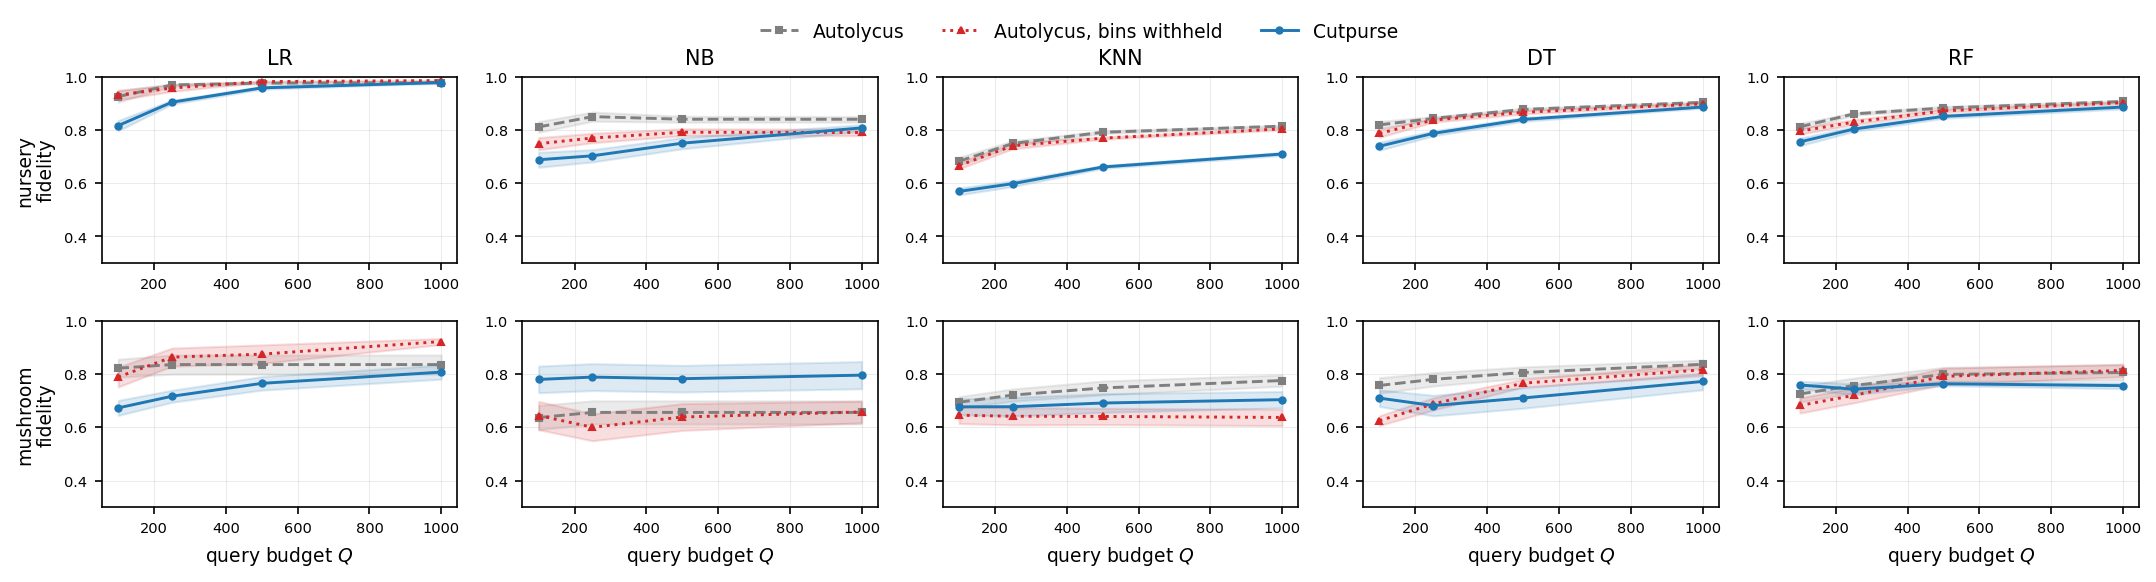
\includegraphics[width=\textwidth]{figures/defense_sweep_categorical.png}
\caption{Defense sweep on the two purely categorical datasets, the companion to
Figure~\ref{fig:defense-sweep}. Withholding the bin edges costs Autolycus almost nothing here, since
integer-encoded categories give the discretizer no meaningful cut points, and \sys\ has no edge to
snap to either.}
\label{fig:defense-sweep-categ}
\end{figure*}

\begin{figure*}[t]
\centering
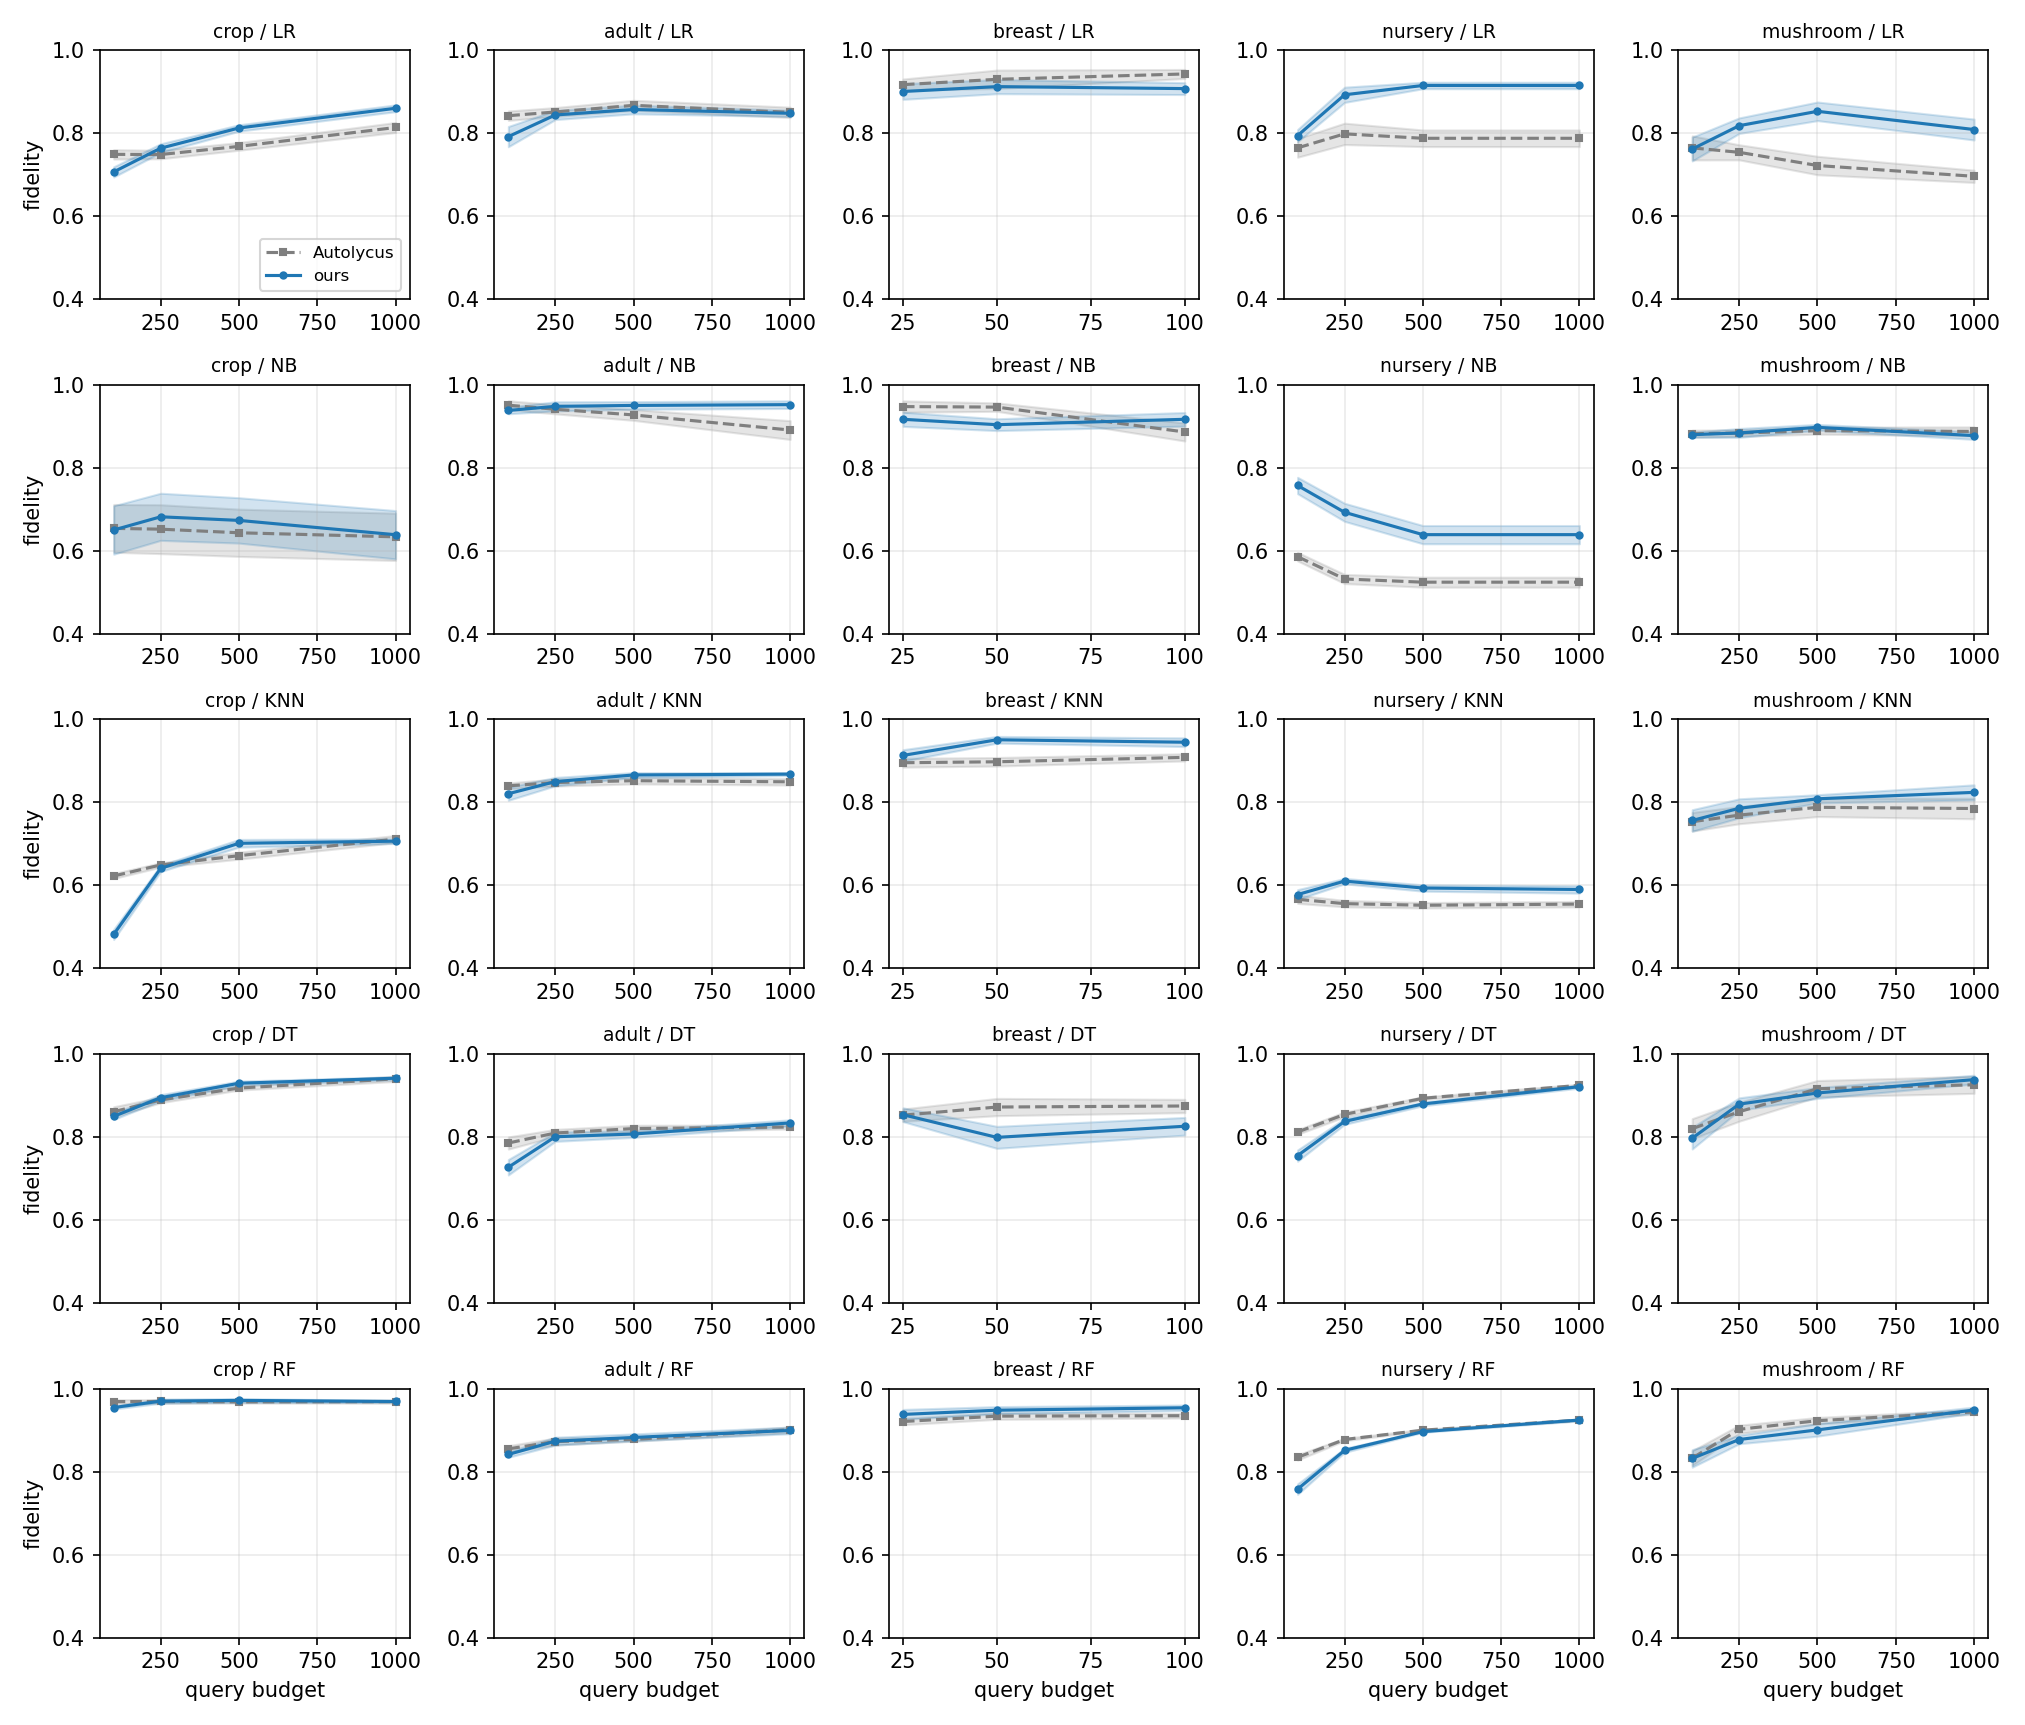
\includegraphics[width=\textwidth]{figures/shap_grid.png}
\caption{\textsc{Shap} companion: surrogate fidelity vs.\ query budget. Our phases reading the target's \textsc{Shap} output
(solid, blue) vs.\ Autolycus-\textsc{Shap} (dashed, grey), per target (rows) and dataset (columns).
Shaded band is the standard error over the $S{=}10$ seed sets; $n{=}5$, $k{=}3$. All panels share a
fixed $y$-axis ($0.4$--$1.0$) for cross-panel comparability.}
\label{fig:shap-headline}
\end{figure*}

Figure~\ref{fig:grid-n3k1} ($k{=}1$, $n{=}3$) shows the largest apparent margin over Autolycus, but
this is an artefact of \emph{base saturation}: at $k{=}1$ Autolycus's traversal exhausts its queue
and cannot spend the budget (its curves go flat), while our diverse generation keeps placing
queries. Figure~\ref{fig:grid-n3k3} ($k{=}3$, $n{=}3$) is the fair control: more seeds, but
Autolycus also uses the full budget. There the mean margin is \emph{smaller} than at $n{=}1$
($+1.9$ vs $+3.4$pp), because additional seeds help Autolycus as much as us. We therefore keep
$k{=}3$, $n{=}1$ as the headline. The larger $k{=}1$ margin reflects Autolycus's budget
under-utilisation, not a seed advantage of our pipeline.

\begin{figure*}[t]
\centering
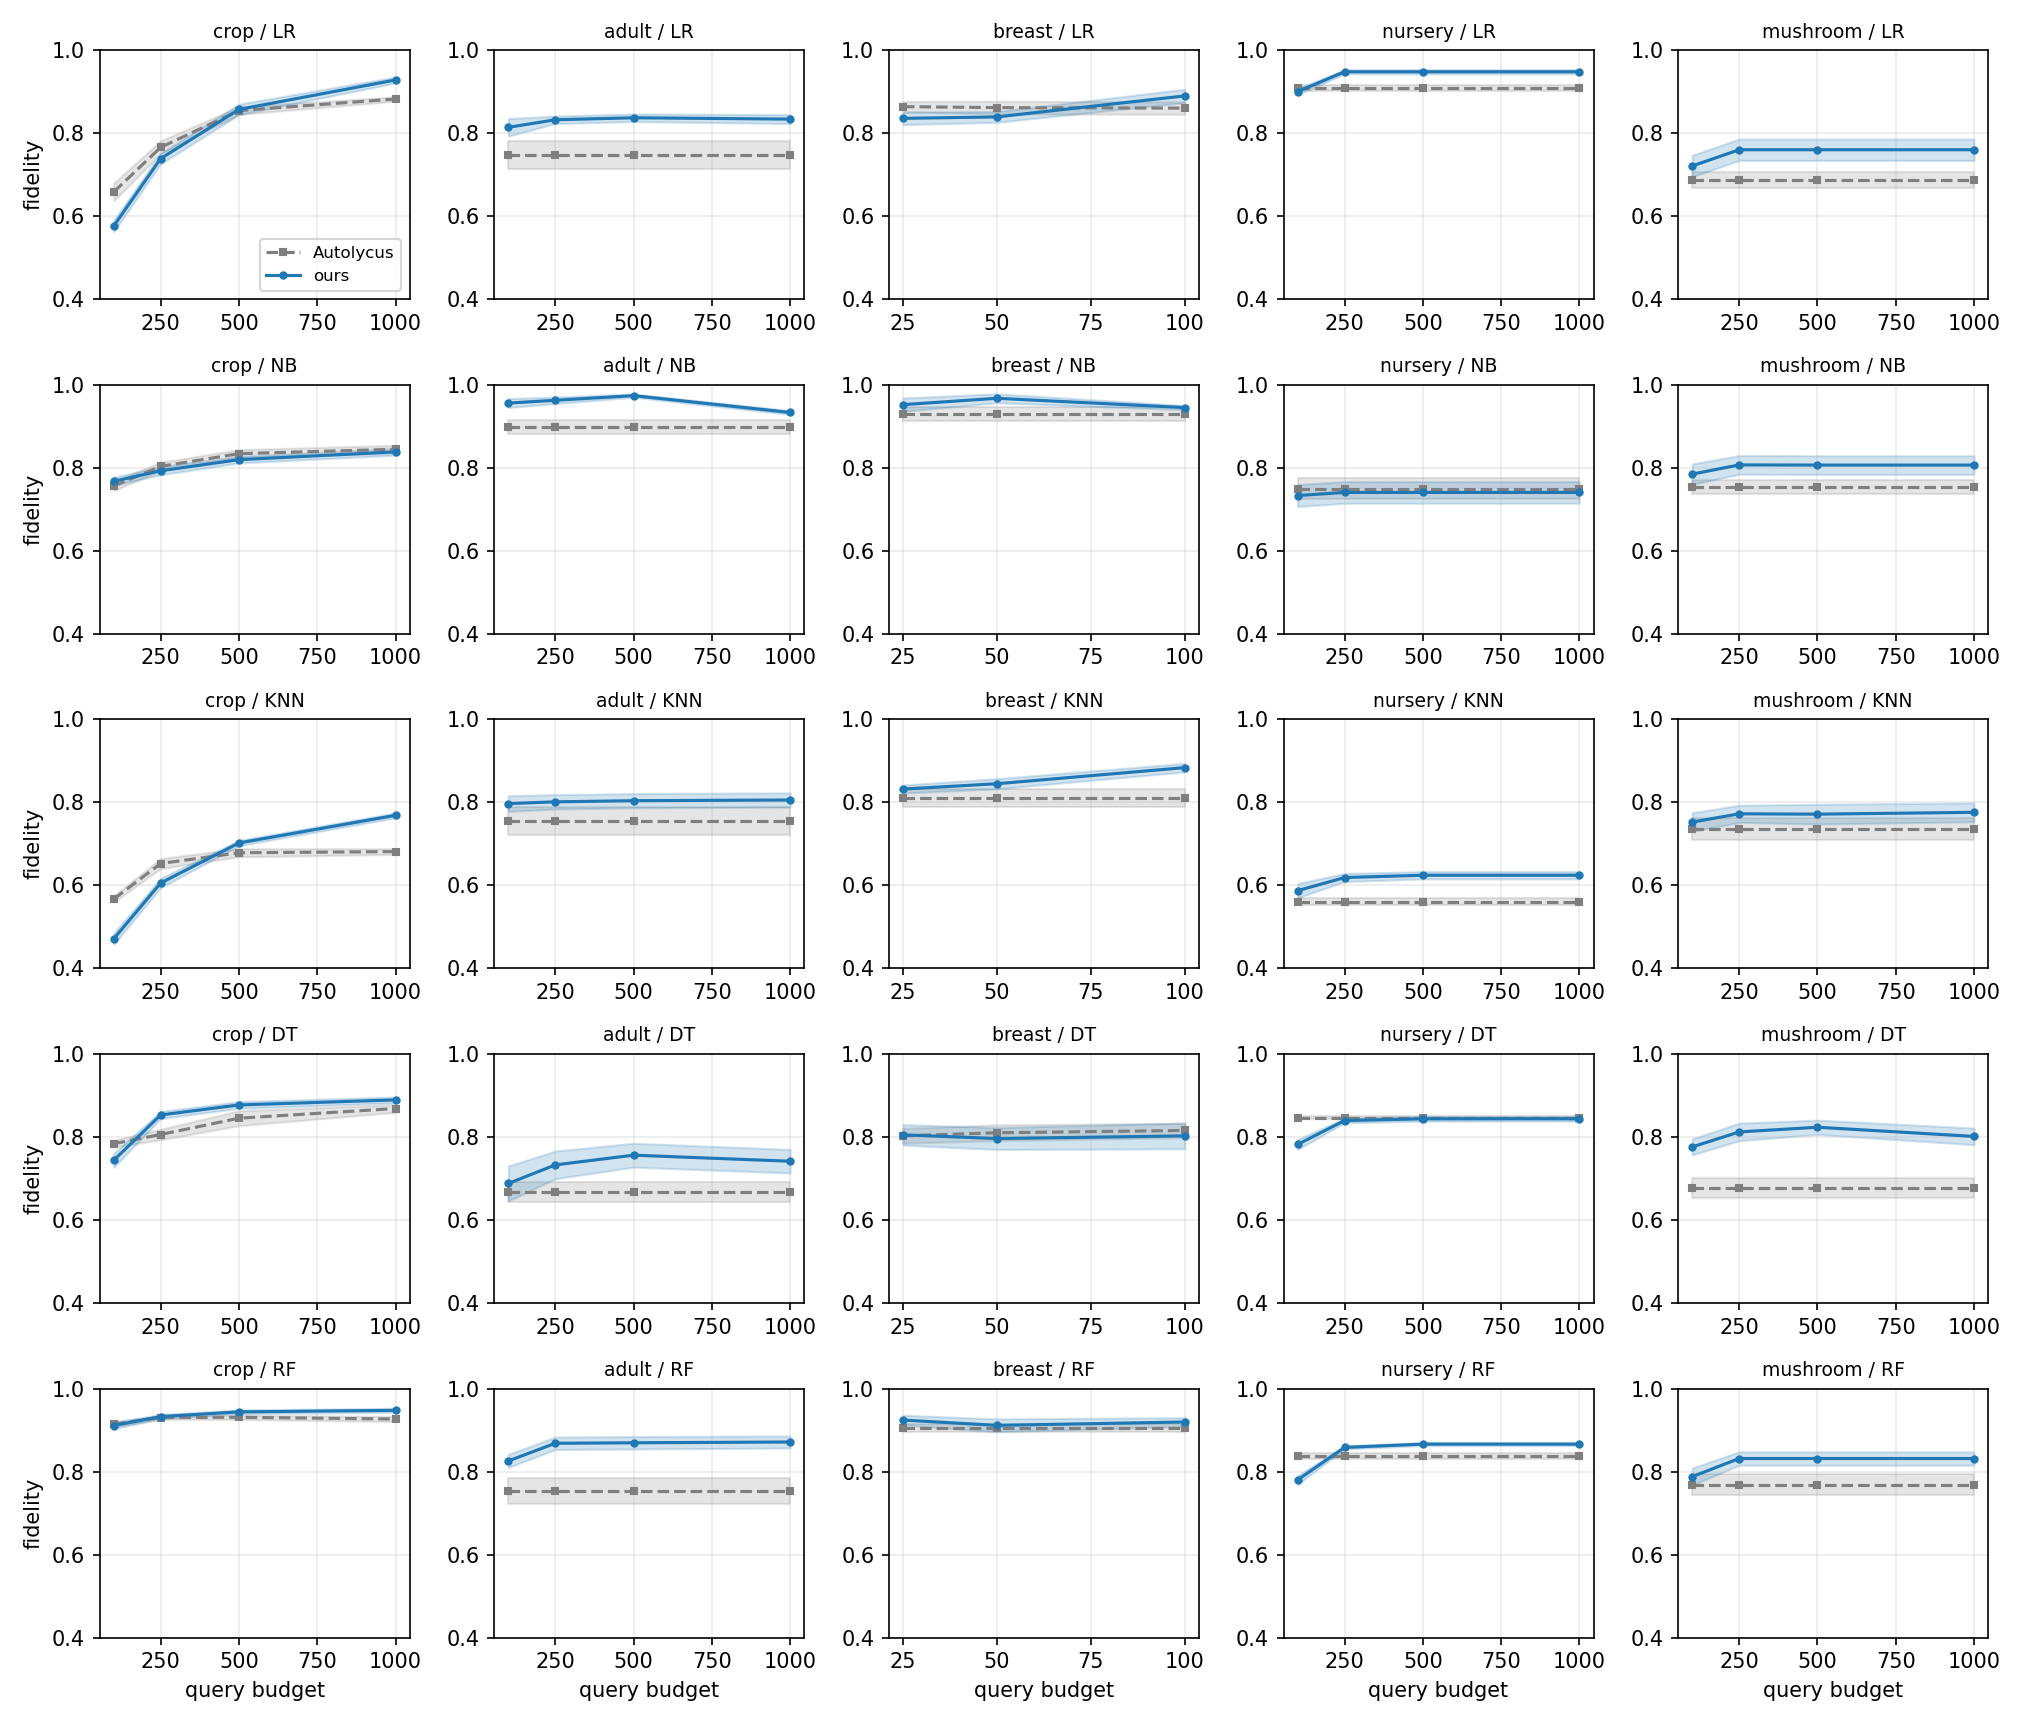
\includegraphics[width=\textwidth]{figures/lime_grid_n3_k1.png}
\caption{LIME at $k{=}1$, $n{=}3$ (secondary). Fidelity vs.\ query budget, ours (blue, solid) vs.\
Autolycus (grey, dashed); band $=$ standard error over 10 sets. Autolycus's curves flatten early because its traversal saturates at $k{=}1$. Shared fixed $y$-axis ($0.4$--$1.0$).}
\label{fig:grid-n3k1}
\end{figure*}

\begin{figure*}[t]
\centering
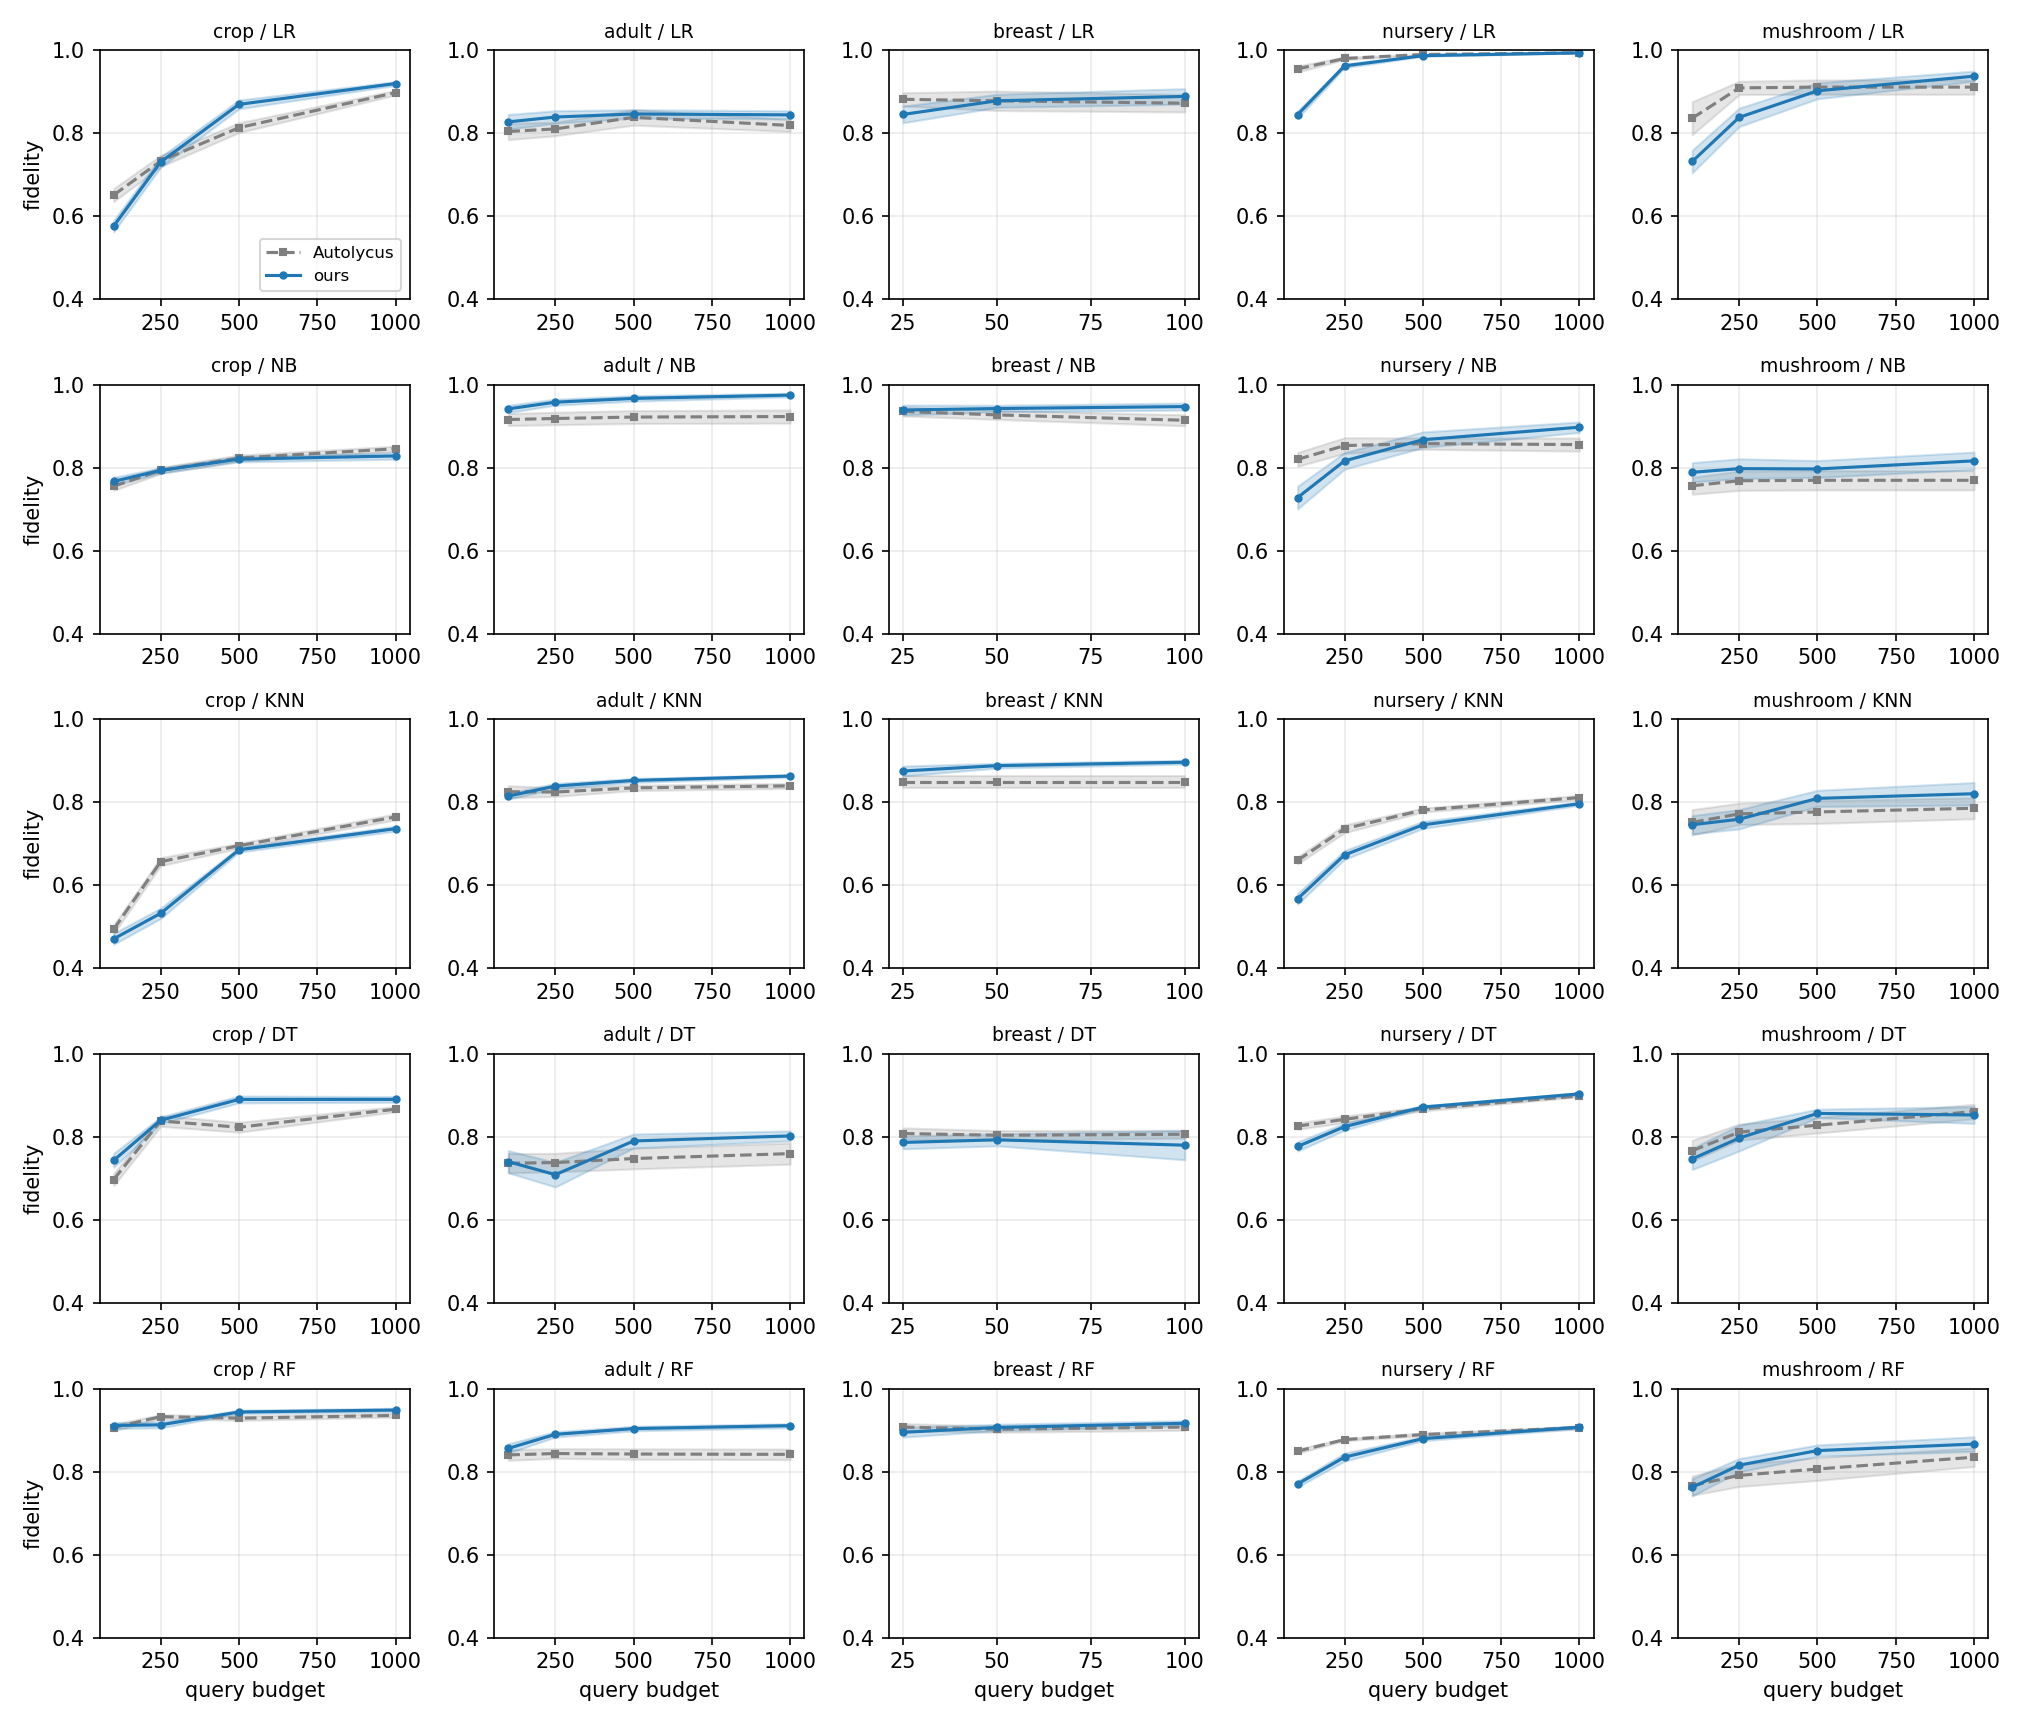
\includegraphics[width=\textwidth]{figures/lime_grid_n3_k3.png}
\caption{LIME at $k{=}3$, $n{=}3$ (fairness control). With $k{=}3$ Autolycus uses the full budget,
and our margin over it is smaller than at $n{=}1$, confirming the larger $k{=}1$ margin is base
saturation, not a seed benefit. Shared fixed $y$-axis ($0.4$--$1.0$).}
\label{fig:grid-n3k3}
\end{figure*}

% Acknowledgements are camera-ready only; omitted under anonymous review.
%\begin{acks}
%\end{acks}

\end{document}
